\documentclass{agasthesis}

\usepackage{geometry}
\usepackage{pstricks}
\usepackage[latin1]{inputenc}
\usepackage[T1]{fontenc}
\usepackage{url}


\graphicspath{{images/}}
\usepackage{amsthm}
\usepackage{graphicx}
\usepackage{ upgreek }
\usepackage{algorithm}
\usepackage[noend]{algpseudocode}
\usepackage{pifont}



%using arcs above letters \overarc
\usepackage{arcs}

%ordentliche nummerierung
\renewcommand*{\thesection}{\arabic{section}}
%gef�llte quadrate bei proof environments 
\renewcommand{\qedsymbol}{$\blacksquare$}



\newtheorem{lemma}{Lemma}[section]
\newtheorem{prop}{Proposition}[section]
\newtheorem{definition}{Definition}[section]
\newtheorem{fact}{Fact}[section]
%\newtheorem{theorem}{Theorem}[section]
\begin{document}
\begin{titlepage}
\enlargethispage{3em}
%%%%%%%%%%%%%%%%%%%%%%%%%%%%%%%%%%%%%%%%%%%%%%%%%%%%%%%%%%%%%%%%%
%%%%%%%%%%%%%%%%%%%%%%%%%%%%%%%%%%%%%%%%%%%%%%%%%%%%%%%%%%%%%%%%%
%%% Kopf mit Logos
\begin{minipage}{0.45\textwidth}
  \begin{flushleft} \small
    
\includegraphics[width=68mm]{Uni-Logo}
    \hspace*{16mm}Fachbereich 4: Informatik
  \end{flushleft}
\end{minipage}
\hfill
\begin{minipage}{0.45\textwidth}
  \begin{flushright} \small
    % hier statt AGAS Logo ggf. Logo einer externen Org. einsetzen
    
\includegraphics[bb=0 40 706 298,height=15mm]{unikorn.eps} \\
    % hier ggf. Namen einer externen Org. einsetzen
    {\ }
  \end{flushright}
\end{minipage}
\vfill
\hspace*{15mm}
\begin{minipage}[b]{0.8\textwidth}
  \begin{flushleft}
  \vspace{2cm}  
%%%%%%%%%%%%%%%%%%%%%%%%%%%%%%%%%%%%%%%%%%%%%%%%%%%%%%%%%%%%%%%%%
%%%%%%%%%%%%%%%%%%%%%%%%%%%%%%%%%%%%%%%%%%%%%%%%%%%%%%%%%%%%%%%%%
%%% hier den Titel der Arbeit eintragen
\LARGE{\bf Reactive Construction of Planar Euclidean Spanners with Constant Node Degree} \\
\vspace{4em}
%%%%%%%%%%%%%%%%%%%%%%%%%%%%%%%%%%%%%%%%%%%%%%%%%%%%%%%%%%%%%%%%%
%%%%%%%%%%%%%%%%%%%%%%%%%%%%%%%%%%%%%%%%%%%%%%%%%%%%%%%%%%%%%%%%%
%%% UNTERTITEL
\Large{
%%%%%%%%%%%%%%%%%%%%%%%%%%%%%%%%%%%%%%%%%%%%%%%%%%%%%%%%%%%%%%%%%
%%%%%%%%%%%%%%%%%%%%%%%%%%%%%%%%%%%%%%%%%%%%%%%%%%%%%%%%%%%%%%%%%
%%% f�r Diplomarbeit
%	Diplomarbeit \\
%	zur Erlangung des Grades \\
%	\textsc{Diplom-Informatiker} \\  % ggf. �ndern zu Diplom-Informatikerin

%%%%%%%%%%%%%%%%%%%%%%%%%%%%%%%%%%%%%%%%%%%%%%%%%%%%%%%%%%%%%%%%%
%%%%%%%%%%%%%%%%%%%%%%%%%%%%%%%%%%%%%%%%%%%%%%%%%%%%%%%%%%%%%%%%%
%%% f�r Studienarbeit
%	Studienarbeit \\

%%%%%%%%%%%%%%%%%%%%%%%%%%%%%%%%%%%%%%%%%%%%%%%%%%%%%%%%%%%%%%%%%
%%%%%%%%%%%%%%%%%%%%%%%%%%%%%%%%%%%%%%%%%%%%%%%%%%%%%%%%%%%%%%%%%
%%% f�r Masterarbeit
%	Masterarbeit \\
%	zur Erlangung des Grades\\
%	\textsc{Master of Science} \\

%%%%%%%%%%%%%%%%%%%%%%%%%%%%%%%%%%%%%%%%%%%%%%%%%%%%%%%%%%%%%%%%%
%%%%%%%%%%%%%%%%%%%%%%%%%%%%%%%%%%%%%%%%%%%%%%%%%%%%%%%%%%%%%%%%%
%%% f�r Bachelorarbeit
	Bachelorarbeit \\
	zur Erlangung des Grades\\
	\textsc{Bachelor of Science} \\
%
im Studiengang Informatik \\
} % end of \Large
%%%%%%%%%%%%%%%%%%%%%%%%%%%%%%%%%%%%%%%%%%%%%%%%%%%%%%%%%%%%%%%%%
\vspace{2em}
\small{vorgelegt von} \\
\vspace{1em}
%%%%%%%%%%%%%%%%%%%%%%%%%%%%%%%%%%%%%%%%%%%%%%%%%%%%%%%%%%%%%%%%%
%%% AUTOR
\Large{
  Tim Budweg
}
\vspace{2em}
%%%%%%%%%%%%%%%%%%%%%%%%%%%%%%%%%%%%%%%%%%%%%%%%%%%%%%%%%%%%%%%%%
%%%%%%%%%%%%%%%%%%%%%%%%%%%%%%%%%%%%%%%%%%%%%%%%%%%%%%%%%%%%%%%%%

%%%%%%%%%%%%%%%%%%%%%%%%%%%%%%%%%%%%%%%%%%%%%%%%%%%%%%%%%%%%%%%%%
%%%%%%%%%%%%%%%%%%%%%%%%%%%%%%%%%%%%%%%%%%%%%%%%%%%%%%%%%%%%%%%%%
%%% BETREUER

  \footnotesize{
      {\bf Betreuer:} M. Sc. Florentin Neumann, Institut f�r Informatik, Fachbereich Informatik, Universit�t Koblenz-Landau \\
      {\bf Erstgutachter:}  Prof. Dr. Hannes Frey, Institut f�r Informatik, Fachbereich Informatik, Universit�t Koblenz-Landau\\ 
      {\bf Zweitgutachter:}  M. Sc. Florentin Neumann, Institut f�r Informatik, Fachbereich Informatik, Universit�t Koblenz-Landau \\
    % hier Abgabemonat und -jahr eintragen
    
    \vspace{1em}
    \begin{flushleft}
    Koblenz, im 11 2015
    \end{flushleft}
 }

  \end{flushleft}
\end{minipage}

\end{titlepage}

\clearemptydoublepage
\thispagestyle{empty}
\ \vfill


\selectlanguage{german}

\section*{Kurzfassung}
Bisher existieren keine beaconlose Algorithmen, welche reaktiv einen planaren euklidischen Spanner produzieren und zugleich konstant ausgangsgradbeschr�nkte Knoten beinhalten.
In dieser Bachelorarbeit werde ich untersuchen, ob die Partial Delaunay Triangulation in Verbindung mit dem Modified Yao Step einen solchen Graph erzeugen kann und es einen Algorithmus gibt, der ihn reaktiv erzeugt.
Dieser Algorithmus hat im Vergleich zur derzeitigen State-Of-The-Art sowohl beim Topologieaufbau als auch beim sp�teren Routing �ber diese Topology einen verringerten Energieaufwand zur Folge, was l�ngere Knotenlaufzeiten erm�glicht.



\section*{Abstract}
Currently, there are no beaconless algorithms which construct planar Euclidean spanners in a reactive way while at the same time providing constant node degree.
This work analysis the approach whether or not the Partial Delaunay Triangulation in connection with the Modified Yao Step can create a graph with all of these properties satisfied and searches for an algorithm which creates this graph in a reactive way.
This algorithm would need less energy than the current state-of-the-art to construct the topology.
In addition, to route messages using that topology leads to a lower energy consumption as well.
This enables nodes to work longer with the same amount of power.

%%%%%%%%%%%%%%%%%%%%%%%%%%%%%%%%%%%%%%%%%%%%%%%%%%%%%%%%%%%%%%%%%
%%%%%%%%%%%%%%%%%%%%%%%%%%%%%%%%%%%%%%%%%%%%%%%%%%%%%%%%%%%%%%%%%
\clearemptydoublepage
\subsection*{Erkl�rung}
Ich versichere, dass ich die vorliegende Arbeit selbst�ndig verfasst
und keine anderen als die angegebenen Quellen und Hilfsmittel benutzt habe
und dass die Arbeit
in gleicher oder �hnlicher Form noch keiner anderen Pr�fungsbeh�rde
vorgelegen hat und von dieser als Teil einer Pr�fungsleistung
angenommen wurde. Alle Ausf�hrungen, die w�rtlich oder sinngem��
�bernommen wurden, sind als solche gekennzeichnet.

Die Vereinbarung der Arbeitsgruppe f�r Studien- und Abschlussarbeiten
habe ich gelesen und anerkannt, insbesondere die Regelung des Nutzungsrechts.
\\[10mm]
\begin{tabular}{p{0.8\linewidth}@{\hspace*{2ex}}r@{\hspace*{2ex}}r}
Mit der Einstellung dieser Arbeit in die Bibliothek bin ich einverstanden.
& ja $\boxtimes $ & nein $\square$ \\[2em] %% change $\square$ to $\boxtimes$ to make a selection
Der Ver�ffentlichung dieser Arbeit im Internet stimme ich zu.
& ja $\boxtimes $ & nein $\square$ \\
\end{tabular}
\\[20mm]

Koblenz, den \today \\[10mm]

%%%%%%%%%%%%%%%%%%%%%%%%%%%%%%%%%%%%%%%%%%%%%%%%%%%%%%%%%%%%%%%%%
%%%%%%%%%%%%%%%%%%%%%%%%%%%%%%%%%%%%%%%%%%%%%%%%%%%%%%%%%%%%%%%%%

%% uncomment for english thesis
\selectlanguage{english}

%% TOC, LOT and LOF
\tableofcontents
\listoftables
\listoffigures

%% include your chapters here
\section{Introduction}
Wireless ad-hoc sensor networks are very useful. 
You can create warning systems for emergency purposes.
For instance, deploying many sensor nodes into the sea or forest to check and caution for tsunamis or fire, respectively.

If a node detects something and sends a message, it is obvious that this message needs to \emph{arrive} at a certain station.
The message should not get lost.
To achieve this guaranteed message delivery in a multi-hop network a specific graph-property called planarity must be satisfied.

Explaining planarity imagine a graph setup watched from above. 
It creates a 2d-view of this graph.
Planarity says that from this view no two edges are allowed to cross each other except in the endpoints.

To planarize a graph some edges must be removed.
If edges are arbitrarily removed from this graph it may result in a disconnected graph or at least randomly long paths.
This needs to be prohibited and can be achieved if a so called \emph{euclidian t-spanner} property is satisfied.
\section{Preamble}
%related work: kanj hat neues ergebnis mit knotenbeschränkung kleiner gleich 11...
%improved local algorithms   2012


%reactive planar spanner
%planar spanner with constant node degree
%

%pdt ist äquivalent zum pudel graph -> on the spanning ratio of pdt

%keine fehler passieren,  nachrichten sofort da sind, keine 4 punkte auf kreis, wenn ich sage dass ein punkt eine nachricht zu einem anderen sendet, ist das ein lokaler broadcast   (alle hören mit, und nur der angesprochene reagiert).

%notations und definitions  -> basics foundations
%danach related work 
\section{Related work}

In the past years several topology controls were invented and further developed.
I am interested in local algorithms only, and hence, centralized algorithms are ignored in this related work.
There are a lot of different approaches with different results.
The following is an extract of these approaches and can be divided into two main groups:
\begin{enumerate}
\item reactive algorithms
\item algorithms which produce a planar t-spanner with constant node degree
\end{enumerate}

Reactive algorithms generally need less messages as only localized algorithms to discover the nodes neighbourhoods due to the lack of beaconing.
They do not need the whole $k $-neighbourhood of every node to function, but only a fractional amount of their direct neighbours.
As time of writing there are three reactive algorithms:
\begin{enumerate}
\item Beaconless Forwarder Planarization (BFP)
\item Guaranteed delivery beaconless forwarding (GDBF) with extension
\item reactive Partial Delaunay Triangulation
\end{enumerate}

First, I will describe an algorithm briefly and in the following there is a short section about properties of the produced graph.
The BFP-algorithm (\cite{Ruhrup2010}) is divided into two phases.
First, in the Selection Phase the executing node $F $ starts the algorithm by sending an RTS. 
In the following every node, which receives this message, starts a timer corresponding to a specific delay function.
The closer a node resides to the executing node, the earlier it answers with a CTS. 
If a node $W $ overhears a CTS of a node $W' $ it checks whether or not it is contained in a certain area corresponding to node $W' $ and $F $.
This area is defined by geometric regions, in the following denoted as $Reg(A, B) $, with $A $ and $B $ being two nodes specifying this region.
The minimum region $Reg(F, W') $ is the Gabriel circle $disk(F, W') $ and the maximum region $Reg(F, W') $ is the Relative Neighbourhood Graph lune over $F $ and $W' $.
The latter describes the area of the intersection of two circles around two neighbouring nodes $UV $ with radii equal to $|UV| $ and with middlepoints $U $ and $V $, respectively.
Different regions cause the algorithm to use different amounts of messages.
This will be discussed later.

Suppose $W $ is contained in such an area it cancels its timer and is, henceforth, called a \emph{hidden node}.
Hidden nodes further participate in the algorithm.
If a hidden node $H $ receives a message from another node $T $, it memorizes this node if $H $ lies in the former defined region. 

The Protest Phase lets hidden nodes protest against violating edges.
An edge $UV $ is called a violating edge if there is a node in $Reg(U, V) $.
If hidden nodes have nodes they memorize they restart the above timer.
As soon as a message from another hidden node $W' $ arrives at hidden node $W $, the latter checks its memorized nodes:
A node $X $ can be removed from the set of memorized nodes if $W' \in Reg(F,X) $.
If the timer of a node expires and there are still nodes which are memorized, the node sends a protest message.
The forwarder node $F $ removes violating edges when it receives protests.

This algorithm performed on each node of a graph $G $ produces a planar subgraph $G' $.
However, $G' $ is not a t-spanner of $G $ and has no constant node degree despite the underlying region ($GG, RNG, CNG $) (refer to ... for an example of these three regions).

$GDBF $ is a scheme to forward messages in a network.
All messages will be greedy forwarded to the node which lies closest to the destination until a node which has no neighbours closer to the destination, called a local minimum, is reached.
From that point a recovery mode is used until the local minimum is exited and the algorithm can switch back to greedy mode.
In greedy mode the message holder broadcasts a RTS-message to all neighbours.
Every neighbour instantiates a timer with length depending on how far the neighbour is away from the destination. 
Nodes closer to the destination answer earlier.
A CTS-message is sent as soon as the timer expires and the message holder forwards the message to its sender. 
Every other nodes cancels its timer and remain silent.
In recovery mode a RTS message from the message holder is as well sent.
Now, all neighbours instantiate a timer corresponding to the distance to the message holder $M $ (closer nodes respond first).
If a neighbour $N $ overhears another nodes $N' $ message, it cancels its timer if $N' \in disk(M, N) $.
For more detailed information, refer to \cite{Chawla2006}.

GDBF can be extended to reactively produce a planar subgraph of a given input graph. 
Since this graph is equal to the Gabriel graph, this is not a t-spanner of the input graph and also has no constant node degree.





%\algrenewcommand\algorithmicprocedure{\textbf{}}
%\begin{algorithm}\small
%\caption{Modified Yao Step}\label{MYS}
%\begin{algorithmic}[0]
%\Statex \textbf{Input:} planar, t-spanner $G $; integer $k\geq 14 $
%\Statex \textbf{Output:} planar, t-spanner $G' $ with constant node degree
%
%\Statex
%
%\For{each node $p\in G $}
%	\State Define $k $ disjoint cones of size $2\pi/k $ around $p $.
%	\State Select for each non empty cone the shortest edge.
%	\For{each maximal sequence $s $ of empty cones}
%		\If{$|s|==1 $}
%			\State Let $nx $ and $ny $ be the incident edges on $p $ clockwise and \State counterclockwise, respectively, from the emtpy cone.
%			\If{either $nx $ or $ny $ has already been selected}
%				\State select the other edge
%				\Else
%				\State Select the shorter edge
%			\EndIf 
%		\Else
%			\State select the first $\lfloor \frac{|s|}{2} \rfloor $ unselected edges incident on $n $ clockwise from $s $
%			\State select the first $\lceil \frac{|s|}{2} \rceil $ unselected edges incident on $n $ counterclockwise from $s $
%		\EndIf
%	\EndFor
%\EndFor
%\State $ G' $ is the subgraph of $G $ consisting of all nodes which are in $G $ and all edges which fulfil that both endpoints of this edge have selected it. 
%\end{algorithmic}
%\end{algorithm}
\section{Algorithm}
This chapter introduces the \emph{reactive Modified Yao Step (RMYS)} and explains it's functionality.
For the sake of completeness follows a scheme of the Modified Yao Step taken from \cite{kanj} and how this can be changed to a reactive approach.
In addition, there is an explanation of how RMYS operates.
Then there is a proof of correctness, followed by an brief analysis of the message complexity and message size of RMYS.
Afterwards, we see which properties the graph produced by RMYS obtains and which not.

\algrenewcommand\algorithmicprocedure{\textbf{}}
\begin{algorithm}\small
\caption{Modified Yao Step}\label{MYS}
\begin{algorithmic}[1]
\Statex \textbf{Input:} planar, connected graph $G $; integer $k\geq 14 $
\Statex \textbf{Output:} planar, connected graph $G' $ with constant node degree of at most $k $

\Statex

\For{each node $p\in G $}
	\State Define $k $ disjoint cones of size $2\pi/k $ around $p $.
	\State Select for each non empty cone the shortest edge.
	\For{each maximal sequence $s $ of empty cones}
		\If{$|s|==1 $}
			\State Let $nx $ and $ny $ be the incident edges on $p $ clockwise and \State counterclockwise, respectively, from the emtpy cone.
			\If{either $nx $ or $ny $ has already been selected}
				\State select the other edge
				\Else
				\State Select the shorter edge
			\EndIf 
		\Else
			\State select the first $\lfloor \frac{|s|}{2} \rfloor $unselected edges incident on $n $ clockwise from $s $
			\State select the first $\lceil \frac{|s|}{2} \rceil $unselected edges incident on $n $ counterclockwise from $s $
		\EndIf
	\EndFor
\EndFor
\Statex $ G' $ is the subgraph of $G $ consisting of all nodes which are in $G $ and all edges which fulfil that both endpoints of this edge have selected it. 
\end{algorithmic}
\end{algorithm}
 
Algorithm \ref{MYS} does not tell, in particular, how this can be computed on a node.
However, my reactive approach, called rMYS, is the following: Since every node knows its PDT-neighborhood (refer to algorithm \ref{RMYS}) which is used by the Modified Yao Step, it can execute this algorithm from line 1 to 14 without further knowledge about it's neighborhood and hence, does not need to send any messages at all.
My approach of RMYS needs to send a RTS-message to each possible neighbor which send a message back if they did not select this edge.
This ensures that only bidirectional edges are used.
Since in most cases the edges are bidirectional a node sends only a so called protestmessage if it did not select an edge and thus, protests against the selection of this edge.

The following algorithm is the definition of RMYS.
For clarity, notice that both acronyms RMYS and rMYS mean \grqq reactive Modified Yao Step\grqq, but former is the algorithm which consists of rPDT, the reactive version of PDT, and rMYS, the reactive way of applying the Modified Yao Step to a planar and connected graph described above.
 
%\textbf{\algrenewcommand\algorithmicprocedure{\textbf{}}
\begin{algorithm}\small
\caption{Reactive Modified Yao Step (RMYS)}\label{RMYS}
\begin{algorithmic}[0]
\Statex \textbf{Input:} any connected graph $G $; integer $k\geq 14 $
\Statex \textbf{Output:} planar, connected graph $G' $ with constant node degree of at most $k $

\Statex

\For{each node $p \in G $}
	\State create the PDT-Neighborhood of $p $ using rPDT
	\State apply rMYS to $p $ using PDT-graph
	\State let each neighbor of $p $ create its RMYS-neighbors and send a protest message if $p $ \indent is not among them causing $p $ to remove this edge
\EndFor 
\end{algorithmic}
\end{algorithm}

\begin{figure}[h!]
\centering
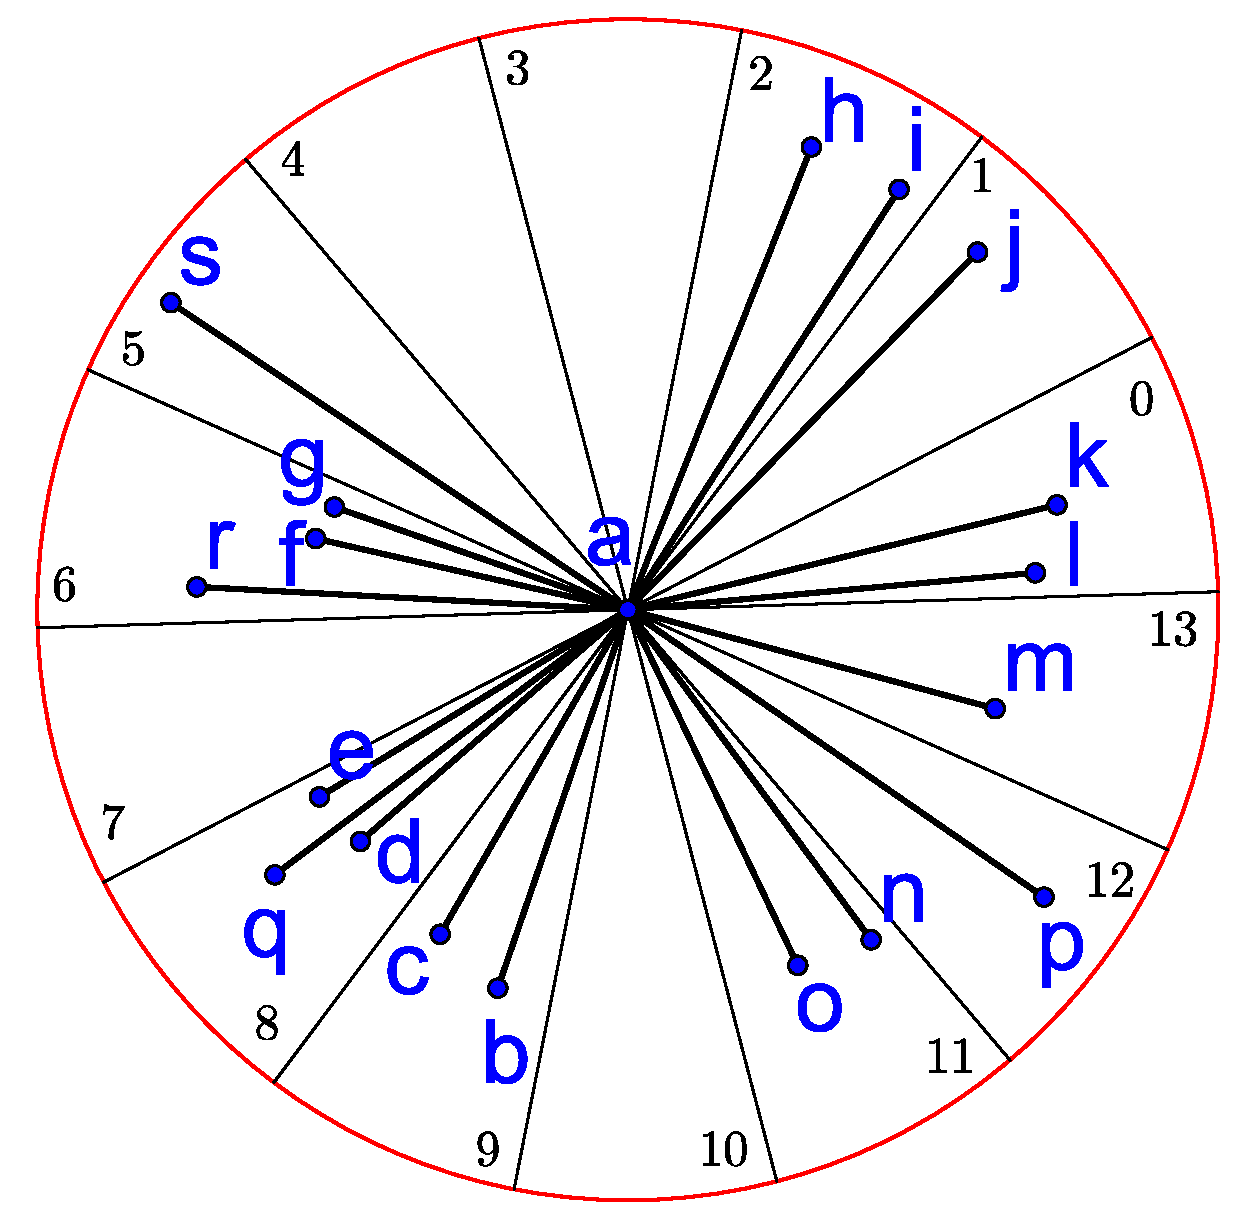
\includegraphics[width=0.6\linewidth]{eps/RMYS_1.eps}
\caption{An example graph and all edges drawn which are incident on $a $. The red circle shows the unit disk of $a $.}
\label{fig:RMYS_1}
\end{figure}

In the following RMYS is presented on the example given by figure \ref{fig:RMYS_1}.
Note that this example calculation is only performed on node $a $.
If one may want to create a complete graph, this algorithm must be executed for every node.

First, create the PDT neighborhood of $a $ using rPTD as explained in chapter \ref{PDT_section}.
Since nodes $p, q, r $ and $s $ are no PDT neighbors of $a $ and, hence they are not needed anymore, they are omitted in the following figures.
Now, the Modified Yao Step starts.
Place $k $ equally sized cones around $a $.
It does not matter where these cones start as long as they start at the same place for all nodes.
For the purpose of this example assume $k=14 $ and that the first cone starts at a horizontal line and runs counterclockwise.
The next step is that $a $ selects for each cone the shortest edge.
In figure \ref{fig:RMYS_2} these steps has been executed.
\begin{figure}[h!]
\centering
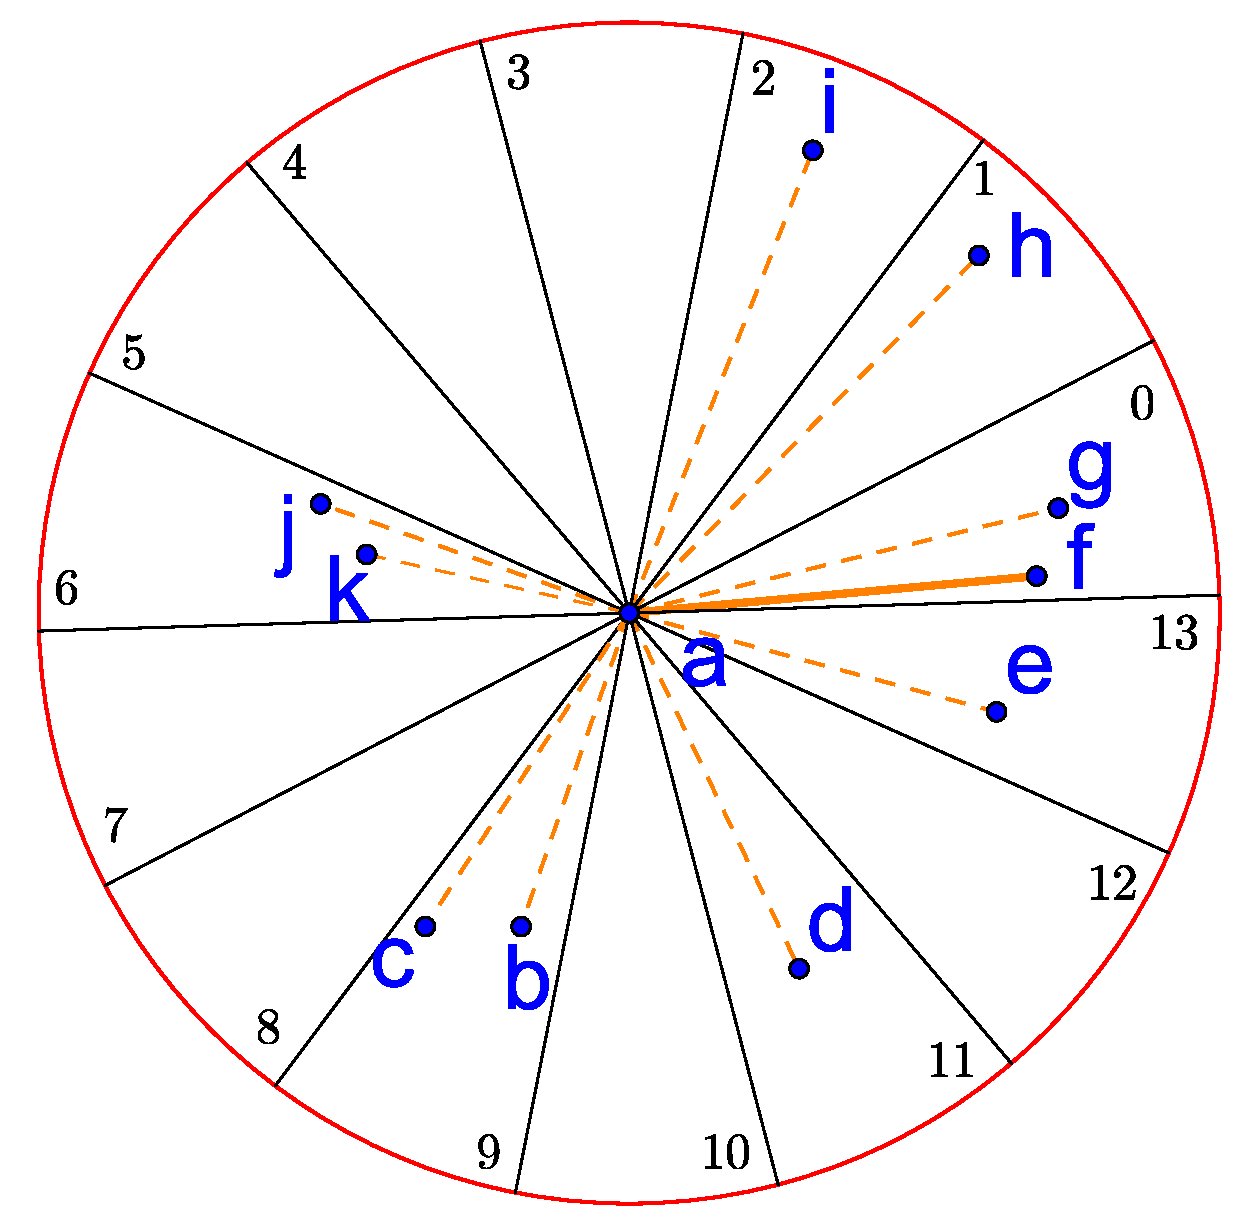
\includegraphics[width=0.6\linewidth]{eps/RMYS_2.eps}
\caption{An example graph with equally sized cones around $a $ and all edges drawn which are incident on $a $. All orange edges has been selected by reason of being the shortest edge in their cone.}
\label{fig:RMYS_2}
\end{figure}
Then, consider all maximal sequences of empty cones.
Let cones $3 $ to $5 $ be the first sequence to be considered.
Select the first $\lfloor \frac{|s|}{2} \rfloor = 1 $ unselected edges clockwise from $s $, with $s $ being the length of the sequence.
Hence, edge $ai $ is selected now.
Counterclockwise the next $\lceil \frac{|s|}{2} \rceil = 2$ unselected edges are selected.
For this reason edges $af $ and $ae $ are additionally selected.
The next empty sequence to analyze is cone 7.
In this case the next edge incident on $a $ clockwise and counterclockwise, respectively, from this cone has to be tested.
Since both edges $ae $ and $af $ are selected yet, no edge will be additionally added.
Moving on, the next empty sequence which is cone 10 must be inspected.
In this example $ao $ is already selected. 
However, $ab $ is not selected yet.
In order to fulfill the algorithm \ref{MYS} it selects $ab $ at this point in time.
The last sequence to analyze is cone 12.
For the same reason as in the sequence before $an $ gets selected.
The last step of the RMYS algorithm is that all of these selected neighbors test whether or not $a $ is also their neighbor.
If this is not the case for one node $z $, this edge is being deleted.
In this example every neighbor accepts $a $ as its neighbor.
Figure \ref{fig:RMYS_3} contains the final graph.

\begin{figure}[h!]
\centering
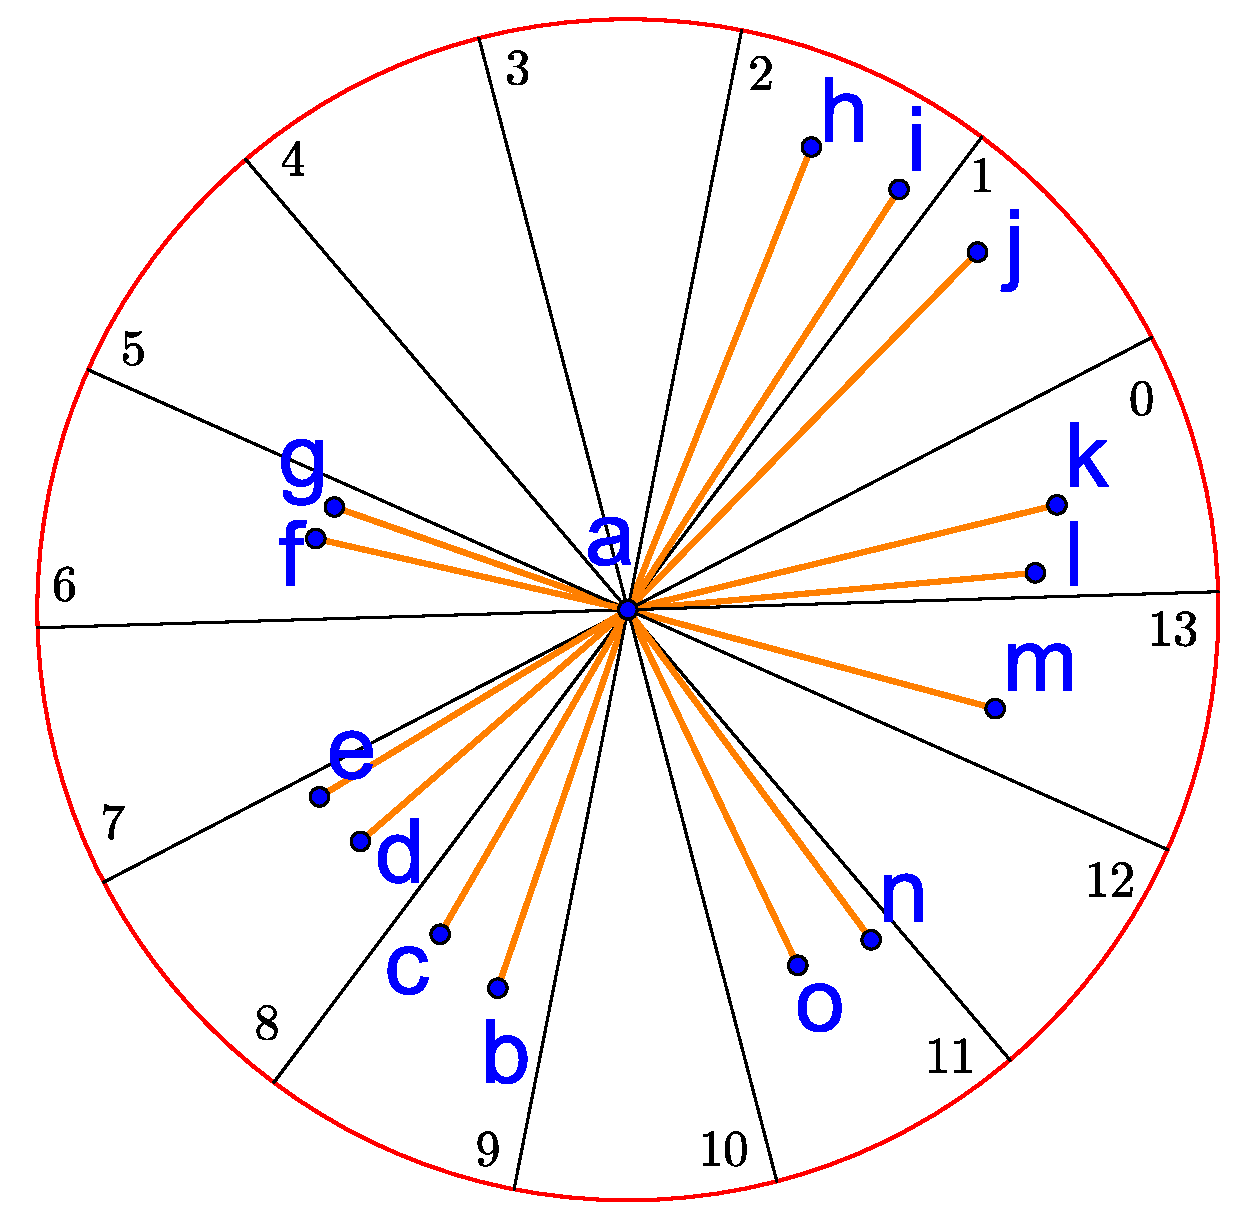
\includegraphics[width=0.6\linewidth]{eps/RMYS_3.eps}
\caption{This is the final graph with all edges drawn in orange which are incident on $a $ after the execution of RMYS.}
\label{fig:RMYS_3}
\end{figure}




\subsection{Proof of correctness}
\begin{proof}
\begin{equation*}
\begin{split}
	MYS(PDT) &\leftrightarrow RMYS\\
	MYS(PDT(v)) &\stackrel{a)}{\leftrightarrow} rMYS(rPDT(v)) \\
    MYS(PDT(v)) &\stackrel{b)}{\leftrightarrow} rMYS(PDT(v))\\
    MYS(PDT(v)) &\stackrel{c)}{\leftrightarrow} MYS(PDT(v)) 
\end{split}
\end{equation*}
We need to proof that the proposed reactive version of this algorithm is equal to a simple concatenation of first, the Partial Delaunay Triangulation and second, the Modified Yao Step on any node $v \in G$.
a) is the fragmentation of the proposition applied to a node $v $.
It is well known that $rPDT $ produces the same graph as the simple local approach, so b) holds true.
$rMYS $ does the same calculation as MYS right before the broadcast in the end.
Therefore, we need only to look at this broadcast.
The executing node $v $ sends a broadcast which must be overheard by all $PDT $ -Neighbors of $v $.
Because of the assumptions that every message arrives and arrives instantaneously, the message cannot get lost.
Every informed node checks whether or not it selects $v $ to be in its RMYS-Neighborhood.
If yes, it remains silent and otherwise it sends a protest message causing $v $ to remove this edge.
Hence, $v $ can check whether or not each node in it's neighborhood accepts this edge.
This leads to the same behavior MYS does and therefore, c) is true and completing this proof.
\end{proof}

\subsection{Message Complexity}
\label{message_complexity}
Let $N_{PDT}(u) $ be the message complexity of $PDT $ creating the neighborhood of Node $u \in G$.
First, $rPDT $ needs at most $n $ messages to create the $PDT $-neighborhood.
Next, the executing node sends at most $k $ messages to its neighbors to ask whether they accept their connection.
At most $k $ answers come back and therefore $k * 2 $.
Every one of this $k $ neighbors needs to calculate it's $PDT $-neighborhood and hence, $k*N_{PDT}(u) $.
The following equation put these reflections into one formula.
\begin{equation*}
\begin{split}
N_{RMYS}(u) &= \underbrace{N_{PDT}(u)}_{\theta (n)} +k *\underbrace{2}_{\theta (1)} + k*\underbrace{N_{PDT}(v)}_{\theta (n)} \\
\theta (N_{RMYS}(u)) &= \theta (n) 
\end{split}
\end{equation*}
Since $k $ is a constant it can be omitted in $O $-Notation.
The sum of the same complexity remains in the same complexity and hence, the message complexity of this algorithm is $\theta (n) $.

\subsection{Message Size}
If the assumption that every node has a unique position holds, this position can be used to identify each node uniquely.
Hence, two floats can be used to save this position resulting in a constant number of bits.
%Other information needed to send are only these node ids or a constant amount of it

\subsection{Properties of the RMYS-graph}
This section is devoted to the graph-properties the RMYS algorithms inherits.
First, it is important to know whether RMYS produces from any connected Unit Disk Graph a connected subgraph.
The first part of RMYS, the Partial Delaunay Triangulation, creates from a connected graph a connected subgraph.
Since rMYS removes edges it may be possible that the graph will be disconnected.
To analyze this we need to recognize that rMYS finds at least one edge per non empty cone.
Since these cones around a node $p $ cover the whole area around $p $ and if there is a node in it, there will be an edge for that cone. %PROOF !! vielleicht einfach
Hence, the graph cannot become disconnected. 

Following this, there is planarity.
The reactive approach of the Partial Delaunay Triangulation produces a planar graph and since the rMYS step of the RMYS-algorithm does not add any edges, the planarity property cannot be violated.
Hence, RMYS produces a planar graph.

Every node has a constant node degree of at most $k $.
First, for each cone the shortest edge is selected.
Resulting in $k $ edges if all cones are not empty.
For all other cases let $l $ be the total number of empty cones.
Then the first step selects $k-l $ edges in all non empty cones and at most $l $ edges are added in the second step.
This leads to a node degree of at most $k $.



\section{Simulation results}
This section is about the simulation results which were achieved.
First, these results are presented.
......
The simulation was performed in Sinalgo\footnote{http://www.disco.ethz.ch/projects/sinalgo/}.
Sinalgo is a simulation framework which can test and validate network algorithms and at the same time it offers a graphical view on the programmed processes as well as a fast batch mode.

There are two different simulation runs.
The first one calculated the Euclidean and hop spanning ratio of PDT and RMYS and the second one counted the messages which were needed to construct PDT, RMYS and the amount of messages needed by two hop beaconing.
1000 random connected graphs for each node density from 5 to 20 were used.
The numbers of nodes $n $ used for each density were calculated with the following formula:
\begin{equation*}
n =round( \frac{D_x \cdot D_y}{\pi \cdot R^2} \cdot density)
\end{equation*}
Hereby, $D_x=1000 $ and $D_y=1000 $ are the dimension of the simulation plane and $R = 100 $ is the unit disk radius.

\bigskip

The simulations are based on the following assumptions.
\begin{itemize}
\item All nodes are static meaning they cannot move.
\item All calculations are ordered into synchronous rounds. 
At the beginning a node receives all messages sent in the round before.
It follows a general calculation phase and at last a node can send messages.
\item Messages arrive instantaneously and cannot get lost.
Every message which was sent, arrives for sure in the round after it was sent.
\item There are no 4 nodes which are co-circular.
\item All graphs are connected.
\end{itemize}

Figure \ref{fig:RMYS_PDT_SpanningRatio} shows the measured spanning ratio of RMYS and PDT to the unit disk graph with respect to node density.
It is noticeable that both lines seem to be the same line.
For density $5 $ the ratio is approximately $1.30 $ and density 20 has approximately a spanning ratio of $1.38 $.
In between 5 and 20 the curve is increasing slightly and has no outliers.

Since both lines are almost identical it is possibly true that RMYS also has a constant spanning ratio which is a fractional amount greater than the proven spanning ratio of PDT (refer to \cite{Neumann2012} for the proven spanning ratio).

\begin{figure}[h!]
\centering
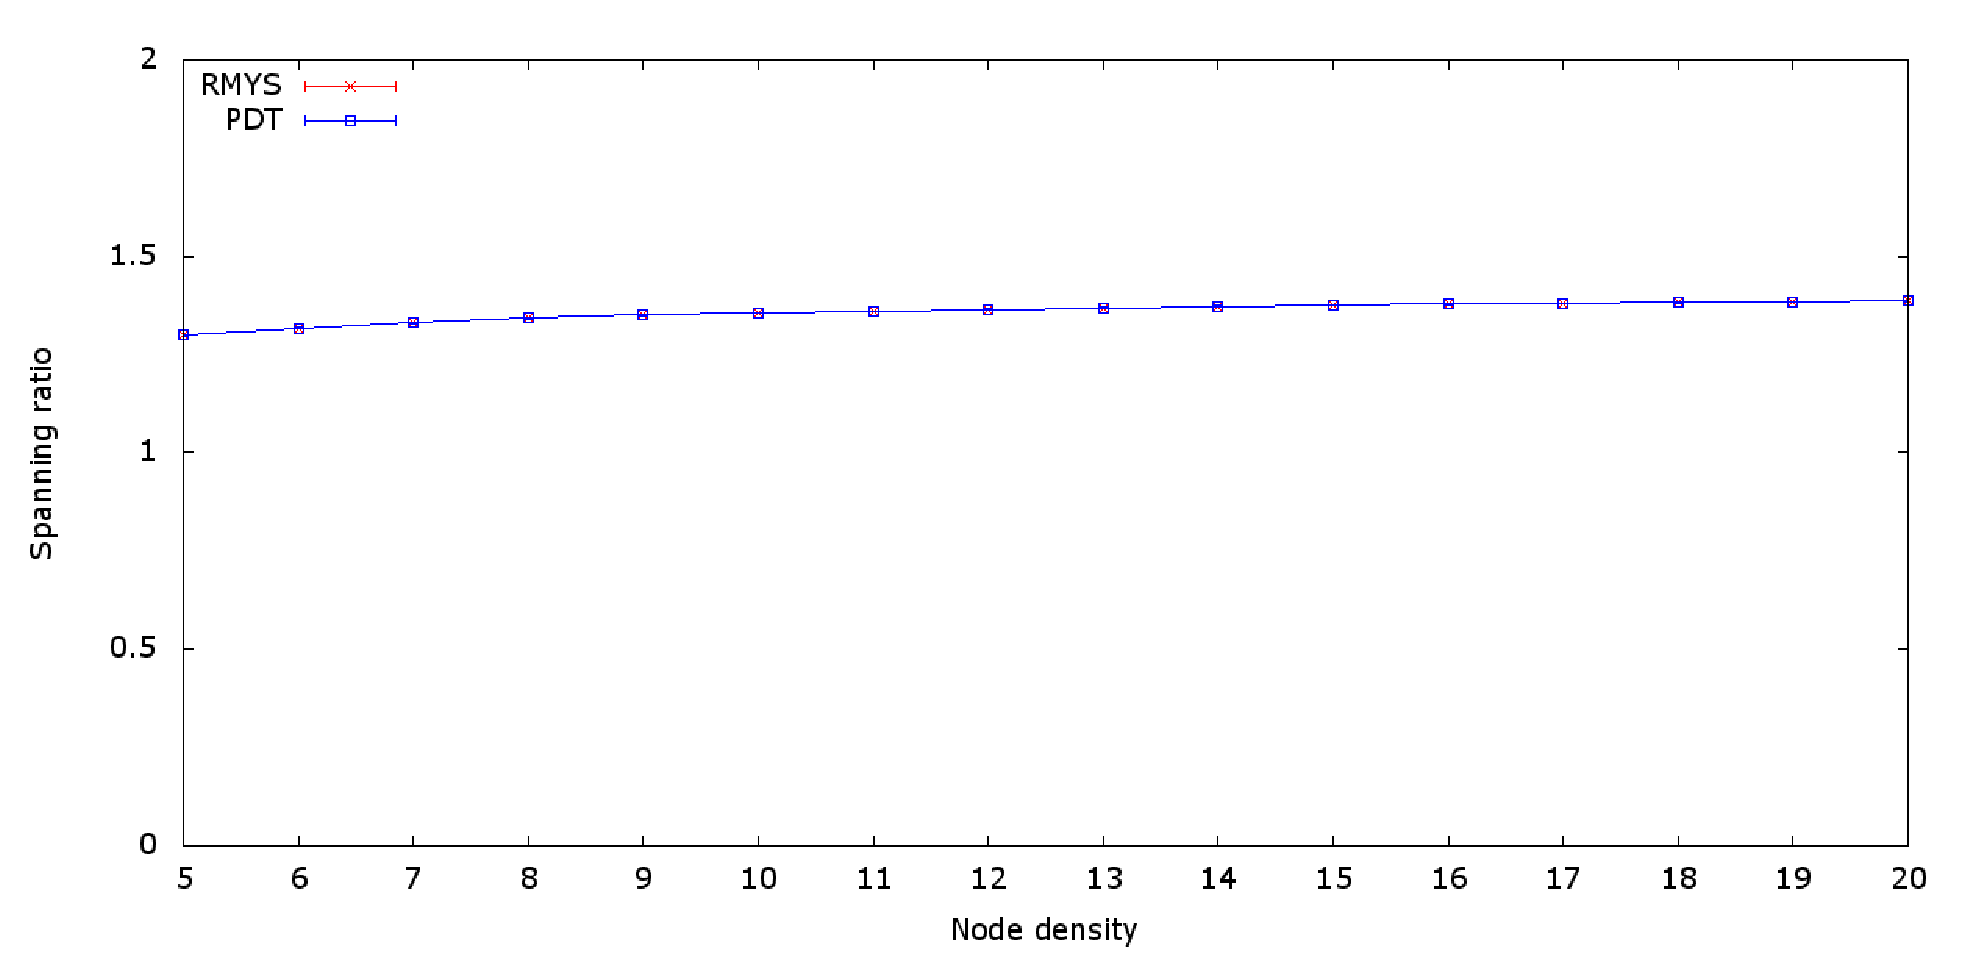
\includegraphics[width=1.0\linewidth]{eps/RMYS_PDT_SpanningRatio.eps}
\caption{Measured Euclidean spanning ratio of Reactive Modified Yao Step (RMYS) and Partial Delaunay Triangulation (PDT) with respect to the unit disk graph in context to the node density. 1000 Simulations per density.}
\label{fig:RMYS_PDT_SpanningRatio}
\end{figure}


Figure \ref{fig:RMYS_PDT_HopSpanningRatio} shows the measured hop spanning ratio of RMYS and PDT to the unit disk graph with respect to node density.
The measured values increase from $3 $ hops at density $5 $ to approximately $4.6 $ at density $20 $.

\begin{figure}[h!]
\centering
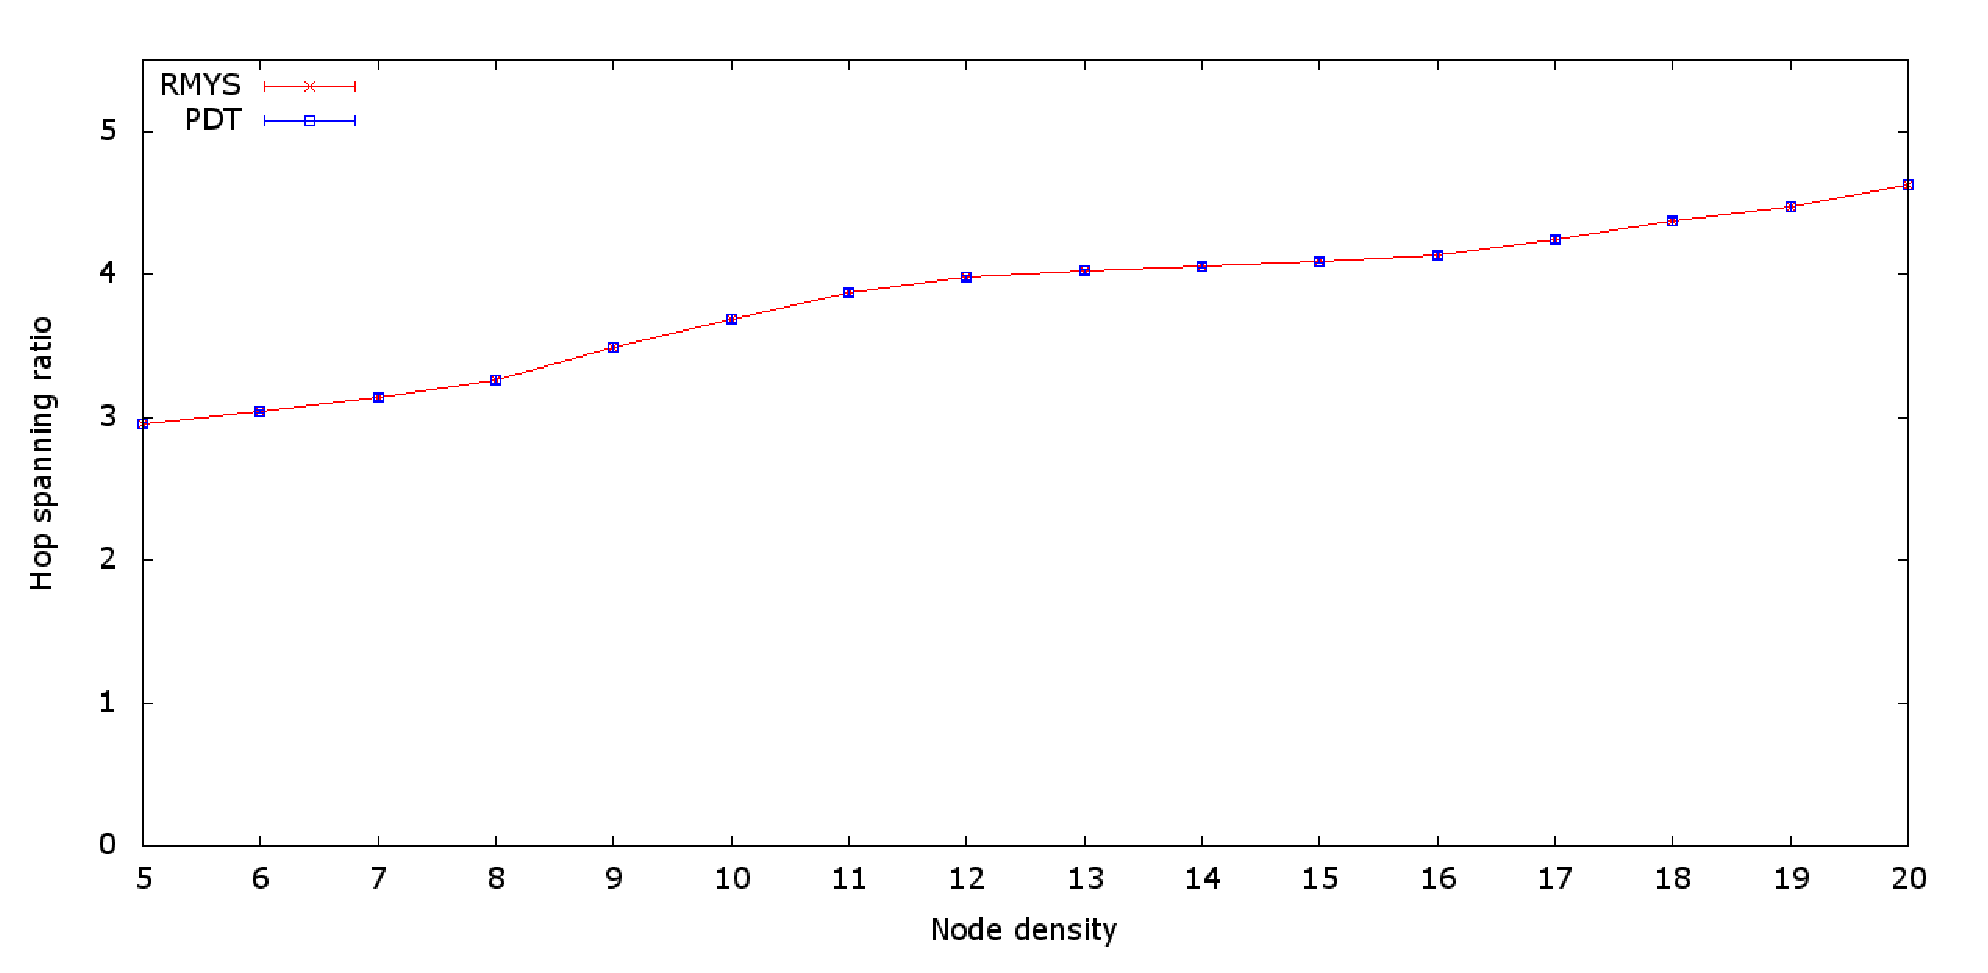
\includegraphics[width=1.0\linewidth]{eps/RMYS_PDT_HopSpanningRatio.eps}
\caption{Measured hop spanning ratio of Reactive Modified Yao Step (RMYS) and Partial Delaunay Triangulation (PDT) with respect to the unit disk graph in context to the node density. 1000 Simulations per density.}
\label{fig:RMYS_PDT_HopSpanningRatio}
\end{figure}



In figure \ref{fig:RMYS_PDT_Beaconing_Neighbors.eps} is the message consumption with respect to node density shown.
"PDT on neighbors" shows the amount of messages PDT uses to create the 2 hop PDT neighborhood of one random node within the graph borders and at least unit disk radius $R=100 $ away from the borders to ensure the correct node density.
In this example the amount of messages RMYS and PDT on neighbors uses are almost equal.
The messages used in 2 hop beaconing are much more.
Additionally, the increase from one density to another is greater than the increase in PDT and RMYS.
At density $5 $ beaconing uses almost twice as much messages as RMYS and at density $20 $ it uses almost tenth times as much messages as RMYS.
For reference, the amount of messages which PDT uses to create the 1 hop PDT neighborhood of the same node as above is shown.
Notice that PDT is message optimal (refer to \cite{Benter2013} for proof) in terms of only nodes which are actually PDT neighbors send messages.

\begin{figure}[h!]
\centering
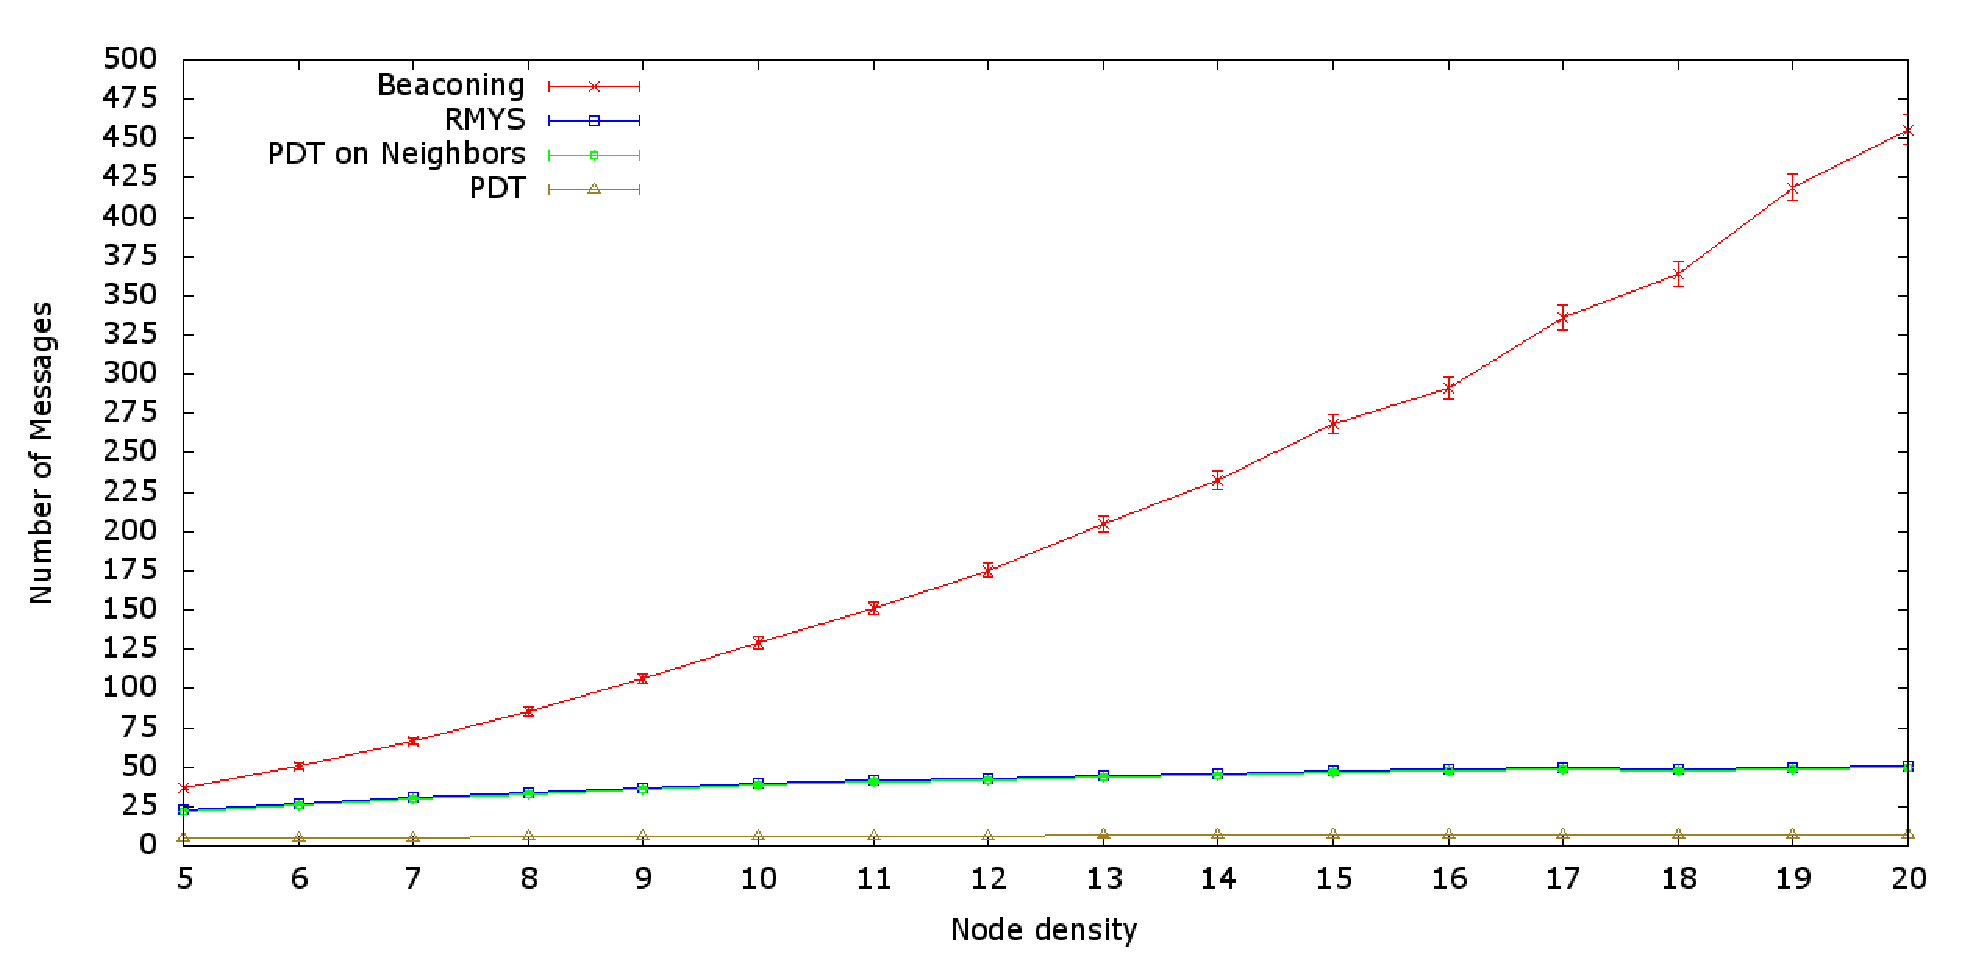
\includegraphics[width=1.0\linewidth]{eps/RMYS_PDT_Beaconing_Neighbors.eps}
\caption{This plot shows the needed messages to construct the RMYS-neighborhood on a given node with respect to the node density in a 2-hop beaconing approach (Beaconing) and in a reactive way (RMYS). Additionally, the messages rPDT uses to construct the PDT-neighborhood of a node (PDT) and its neighbors (PDT on Neighbors) are shown. 1000 Simulations per density.}
\label{fig:RMYS_PDT_Beaconing_Neighbors.eps}
\end{figure}

Figure \ref{fig:RMYS_PDT_Neighbors} shows the message consumption with respect to node density between RMYS and PDT on neighbors in order to notice the small differences.
In fact RMYS uses always one message more than PDT on neighbors.
For reference, the message consumption for PDT on one node is shown as well.

\begin{figure}[h!]
\centering
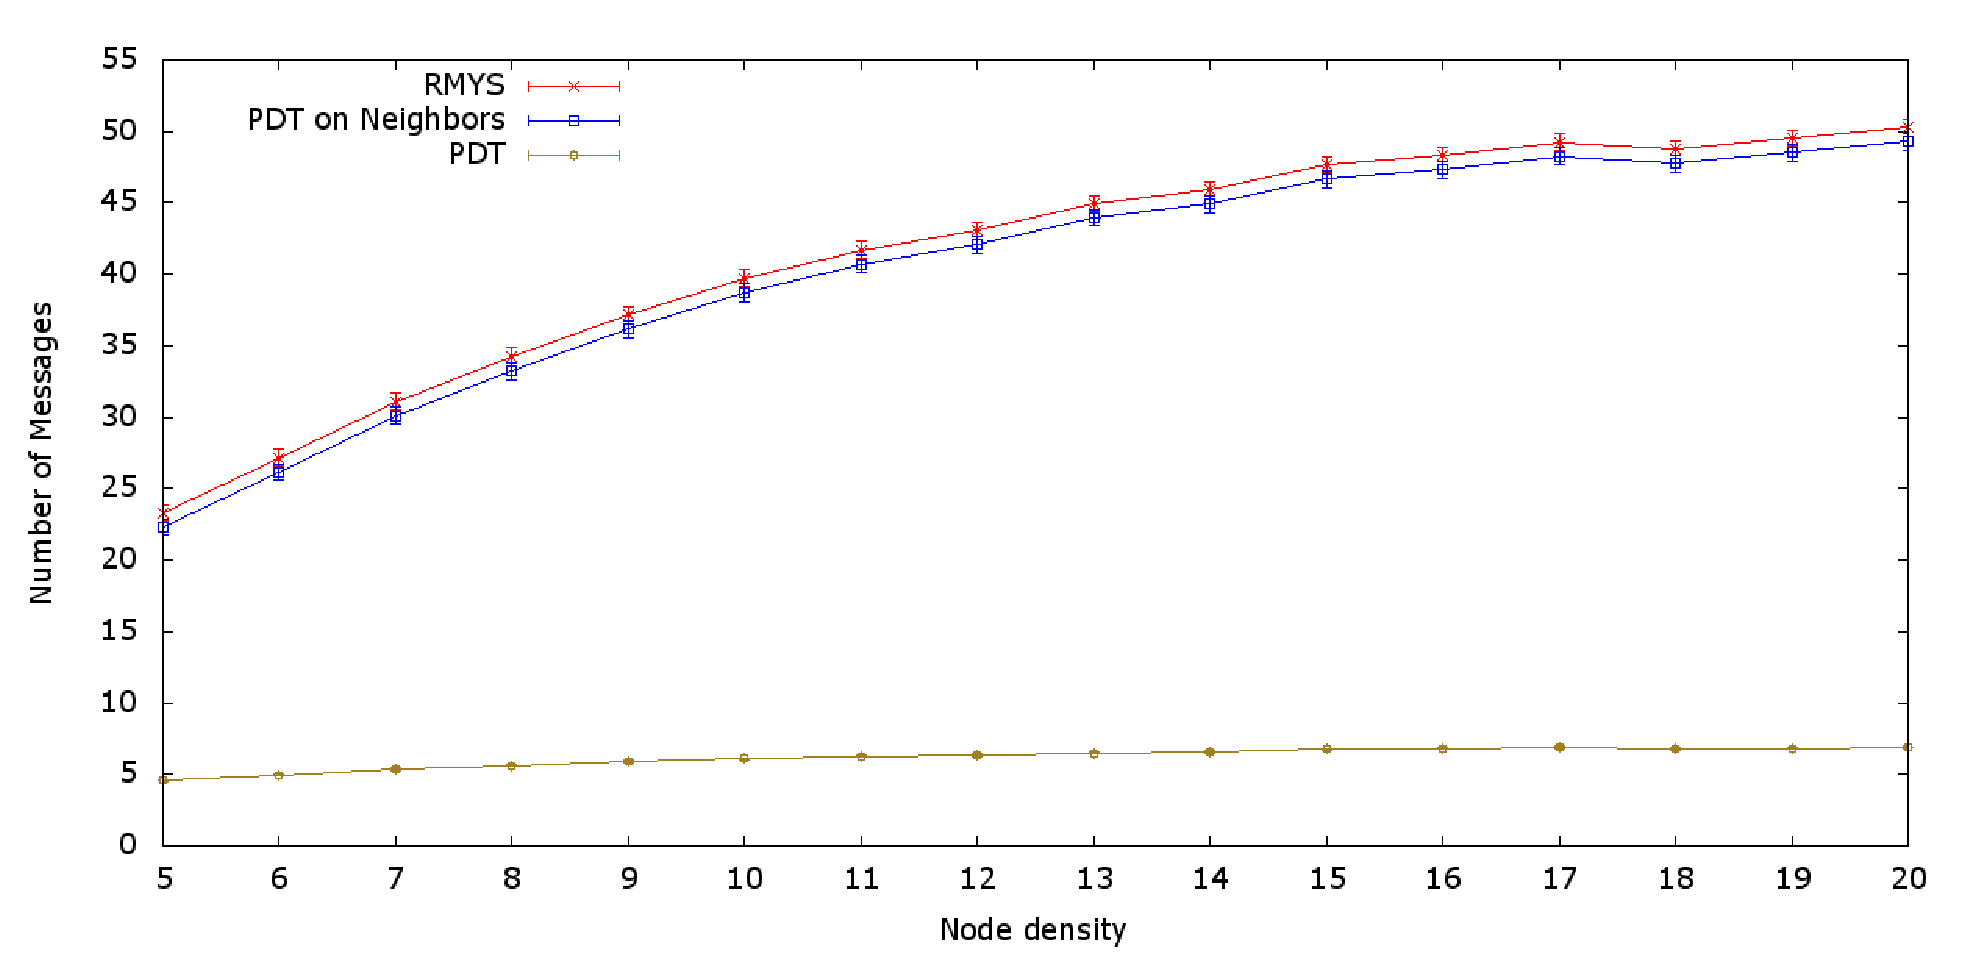
\includegraphics[width=1.0\linewidth]{eps/RMYS_PDT_Neighbors.eps}
\caption{The messages needed to construct the PDT-neighborhood of a node (PDT) and its neighbors (PDT on Neighbors) are shown. Additionally, the message usage of the RMYS neighborhood creation is visualized. 1000 Simulations per density.}
\label{fig:RMYS_PDT_Neighbors}
\end{figure}


Refer to figure \ref{fig:RMYS_PDT_avrNeighbors} to see the average and maximal neighbors of the RMYS and the PDT graph.
Density $5 $ leads to approximately $3.6 $ neighbors and almost $6 $ neighbors at density $20 $.
The maximal neighbors differ for both graphs from $6.89 $ at density $5 $ to approximately $10.35 $ for RMYS and $10.44 $ for PDT at density $20 $.
The differences of the maximal neighbors for RMYS and PDT at high densities is explained in REF.

\begin{figure}[h!]
\centering
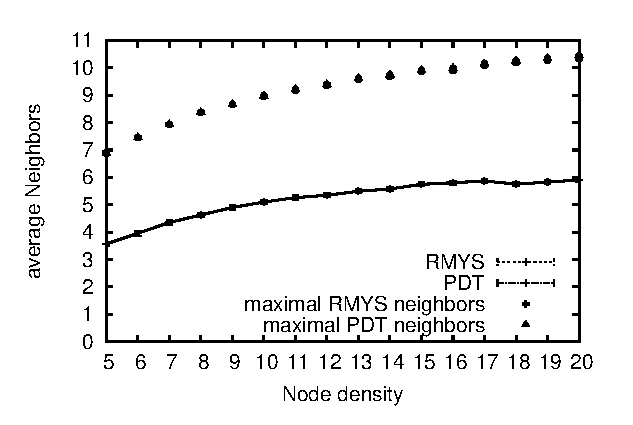
\includegraphics[width=1.0\linewidth]{eps/RMYS_PDT_avrNeighbors.eps}
\caption{Average and maximal Neighbors of Reactive Modified Yao Step (RMYS) and Partial Delaunay Triangulation (PDT) with respect to node density. 1000 Simulations per density.}
\label{fig:RMYS_PDT_avrNeighbors}
\end{figure}


Figure \ref{fig:RMYS_PDT_UDGNeighborsRatio} shows the amount of neighbors in the subgraphs RMYS and PDT of a random node divided by the amount of neighbors in the unit disk model of the same node.
A value of $1 $ corresponds to all unit disk neighbors are neighbors in the subgraph.
At density $5 $ approximately $0.8 $ percent of all unit disk neighbors are PDT and RMYS neighbors.
At density $20 $ this percentage dropped to $0.33 $.

\begin{figure}[h!]
\centering
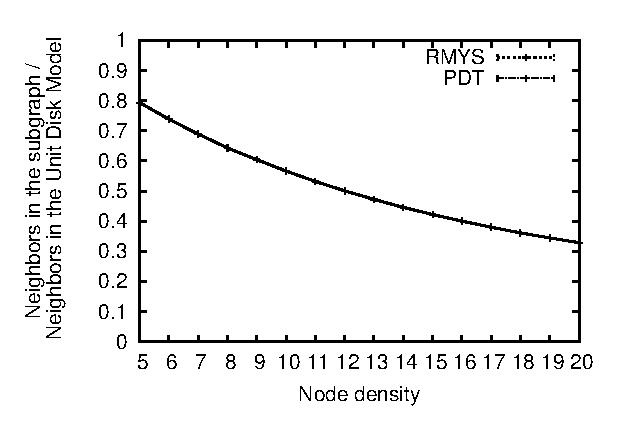
\includegraphics[width=1.0\linewidth]{eps/RMYS_PDT_UDGNeighborsRatio.eps}
\caption{The average neighbors for Reactive Modified Yao Step (RMYS) and Partial Delaunay Triangulation (PDT) divided by the average neighbors in the unit disk model are shown. 1000 Simulations per density.}
\label{fig:RMYS_PDT_UDGNeighborsRatio}
\end{figure}

\begin{figure}[h!]
\centering
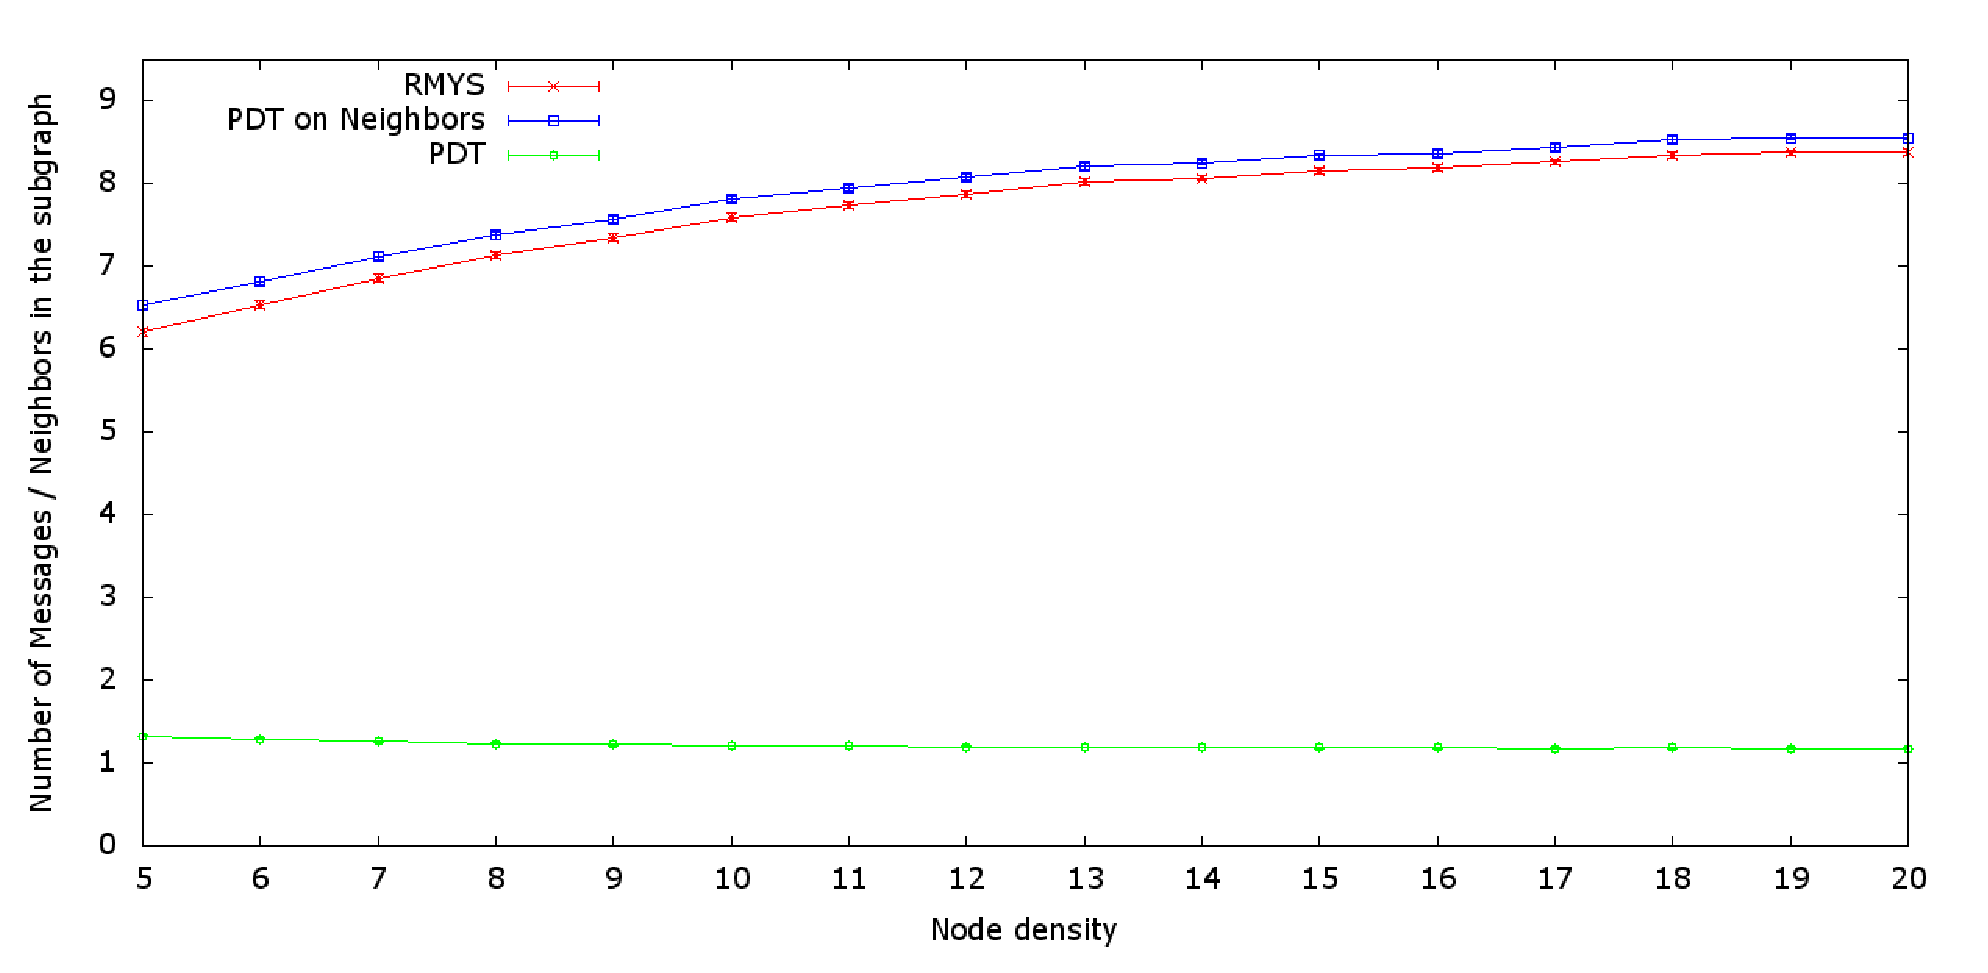
\includegraphics[width=1.0\linewidth]{eps/RMYS_PDT_MessagesPerNeighbors.eps}
\caption{The messages needed to construct the RMYS neighborhood (RMYS), the PDT neighborhood of a node (PDT) and its neighbors (PDT on Neighbors) divided by the actual neighbors in this subgraph are visualized. 1000 Simulations per density.}
\label{fig:RMYS_PDT_MessagesPerNeighbors}
\end{figure}

In Figure \ref{fig:RMYS_PDT_MessagesPerNeighbors} is the number of used messages by a topology control divided by the obtained neighbors in the specific subgraph visualized.
Here, $1 $ corresponds to for each neighbor in the subgraph $1 $ message was sent.
PDT uses not much more than this.
At density $5 $ PDT sends approximately $1.33$ and at density $20 $ approximately $1.18 $ messages per neighbor.
PDT on neighbors and RMYS send $6.2 $ and $6.5 $, respectively, messages per neighbor at density $5 $.
At density $20 $ PDT on neighbors uses $8.4 $ and RMYS $8.6 $ messages per neighbor.

\section{Discussion}
In the following the simulation results are interpreted and explained.
Additionally, 
There are two cases where RMYS does not select all neighbors of a node, even if the count of these neighbors is below the limit of $k=14 $.
Both cases are presented briefly in the following.
First, notice figure \ref{fig:RMYS_ErrorBiderectionalEdges}.
This figure contains two nodes $u $ and $v $ with one of their RMYS cones drawn.
The blue circles and the dotted line marked with $R $ symbolize the unit disk radius of both nodes.
The green circle proofs that $uv $ is a PDT edge.
Suppose that the red area contains a node $n $ and that any other cone of $v $ (not visualized) contains also one node.
If RMYS is executed on that example, $u $ selects $v $ in any case since it is the only node in that cone.
However, $v $ selects $n $ since it is closer to $v $ than $u $.
All other cones contain nodes as well and therefore no more edges are selected.
As a result of this behavior the edge $uv $ was selected from only one, namely $u $, of its endpoints and therefore, $v $ sends a protest message.

\begin{figure}[h!]
\centering
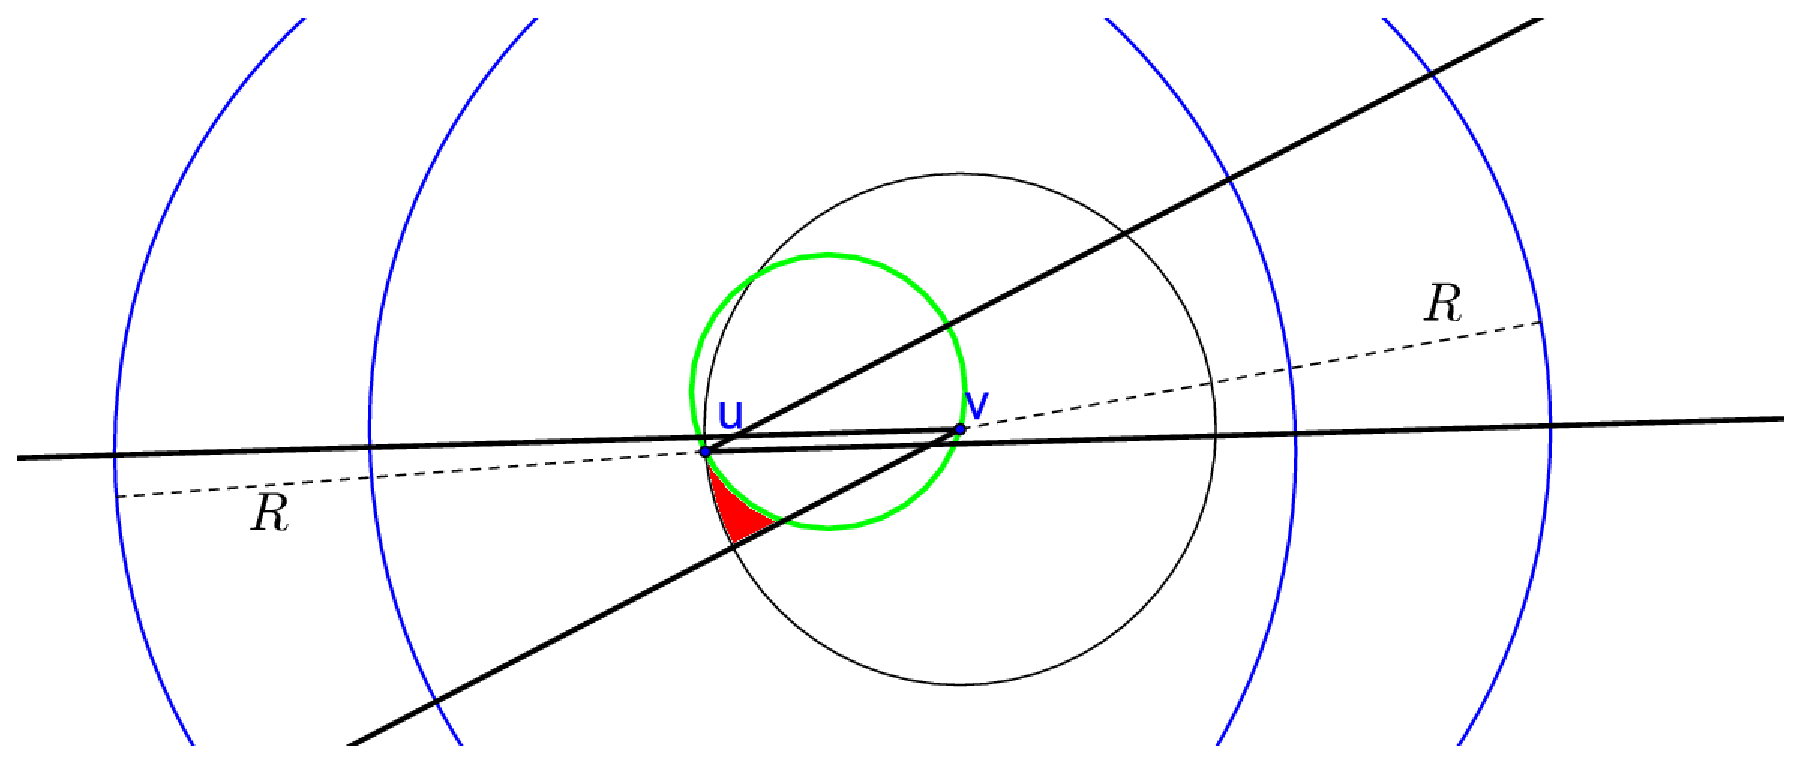
\includegraphics[width=1.0\linewidth]{eps/Zwei_Punkte_mit_RMYS_KEGEL.eps}
\caption{Node $u $ and $v $ are drawn with a specific cone and blue unit disk circles with radius $R $. The green circle is the PDT circle for edge $uv $ and if the red area contains a point, $uv $ is no bidirectional RMYS edge.}
\label{fig:RMYS_ErrorBiderectionalEdges}
\end{figure}

An example for the second case can be viewed in figure \ref{fig:RMYS_case_one_cone_empty.}.
It shows a view on an example graph with all edges incident on $v $ drawn.
In addition, the Gabriel circles of some nodes is visualized in a dotted way.


The maximal neighbors in above mentioned figure were calculated above all nodes in a graph and on some rare occasions these cases happened.
In order to understand the small deviation of maximal neighbors at high densities between RMYS and PDT in figure \ref{fig:RMYS_PDT_avrNeighbors} see 


\begin{figure}[h!]
\centering
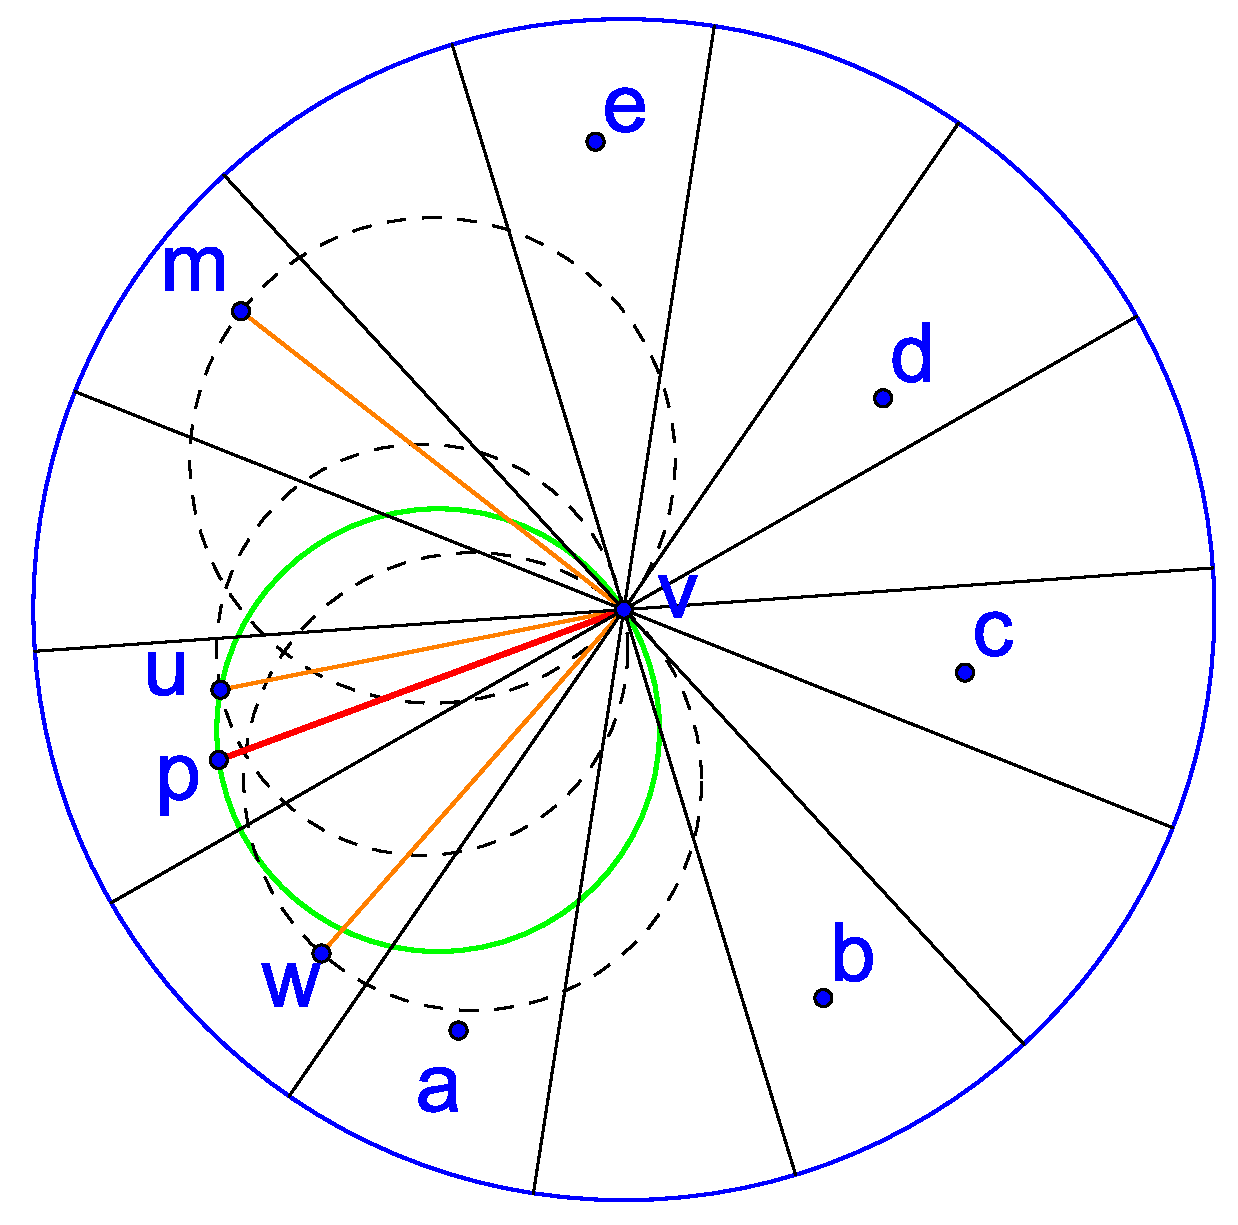
\includegraphics[width=0.8\linewidth]{eps/RMYS_case_one_cone_empty.eps}
\caption{}
\label{fig:RMYS_case_one_cone_empty}
\end{figure}


\section{Proof}
Let U be the Unit Disk Graph of the Euclidean Graph of a Node Set S.
The authors of \cite{kanj} use $LDel^{(2)}(U) $ as the underlying subgraph of the Modified Yao Step.
$LDel^{(2)}(U) $ is defined as the union of the Gabriel-graph and the subgraph of U in which the circumcircle of every triangle does not contain a 2-hop-neighbor of the nodes which create the triangle.
However, it is not known whether $LDel^{(2)}(U) $ can be constructed reactively.
At this point I want to introduce the \emph{Partial Delaunay Triangulation (PDT)} \cite{pdt} which might be a valid replacement.
The following part of this work will examine the possibility of this replacement and, thus, proving the correctness of the following proposition:

\begin{prop}
\label{mastertheorem}
For every integer $k \geq 14 $, there exists a sugraph $G' $ of $G $ such that $G' $ has maximum degree k and stretch factor $1+2\pi (k*\cos{\frac{\pi}{k}})^{-1} $.
\end{prop}

At first, note that the style of this proof is adapted from \cite{kanj}.\\
In a style similar to the definition of $LDel^{(2)}(U) $ from \cite{kanj}, we define the Partial Delaunay Triangulation as follows:
\begin{definition}
\label{emptycircle}
An edge XY of U is contained in the PDT graph if and only if there exists a circle trough X and Y whose interior contains no point of U that is a 2-hop neighbor of X or Y.
\end{definition}
\begin{proof}
This can be verified since the original PTD-Definition from \cite{pdt} is defined like above, except that the circle must not contain \emph{any} nodes of U. 
If this region contains no nodes at all, it cannot contain nodes which are 2-hop-neighbors of X or Y either.  
\end{proof}

Additionally, the following Delaunay Graph property is being used:
\begin{lemma}
\label{emptyregion}
If CA and CB are edges of the PDT graph then the region of $(O)=\bigcirc{ABC} $ subtended by chord  CA and away from B and the region of $(O) $ subtended by chord CB and away from A contain no points that are two hop neighbours of A, B and C.
\end{lemma}


See Figure \ref{fig:empty_region} for a graphical illustration of the above lemma.
This property also holds true for PDT.

\begin{proof}
Since $CA $ is a PDT edge there is a circle $\bigcirc{c_1} $ with C and A on it's border which does not contain any node (so non two-hop-neighbour of C or A, either) of U.
Suppose we take another third Point d, which is not in the Set U, to identify $\bigcirc{c_1} $.
No matter where the third point d of this circle is placed, the region, in the following named $R_1 $, of $\bigcirc{ABC} $ delimited by chord $CA $ away from B is always contained completely in $\bigcirc{c_1} $ and, therefore, empty.

The next part proofs this proposition.
By symmetry of circles it is sufficient to put d on a line  $l $ which is defined as the perpendicular bisector of $CA $.
Let $\alpha<\pi $ be the smaller angle in $\angle{AdC} $.
If d moves on the line $l $ the angle $\alpha $ changes.   
Let $\beta >0$ be the value of alpha, when $B $ is on the border of circle $\bigcirc{c_1} $.
Let d start at degree $\alpha = \pi-\epsilon $ for $\epsilon $  arbitrarily small but greater than $0 $.
Since d is continuous in the interval $[\beta,\pi[ $, every possible circle is covered:
\begin{itemize}
\item If $\alpha $ is barely equal to $\pi $, d is located at the nearest position to edge $CA $ on $l $.
\item If $\alpha=\beta $ is satisfied, $B $ is on the border of $\bigcirc{c_1} $.
\item If $\alpha <\beta $ is satisfied, $B $ is contained in the circle and hence, this is not a valid circle.
\end{itemize}
Suppose $c_1 $ is the Gabriel circle ($\alpha=\frac{\pi}{2} $).
Then $R_1 $ is contained in $c_1 $. 
If $\alpha $ is a value in $[\frac{\pi}{2},\pi[ $ the circle $c_1 $ expands on the side of $CA $ on which $R_1 $ is located which means that $R_1 $ must still be inside $c_1 $.
If $\alpha $ is a value in $]\frac{\pi}{2},\beta[ $ the circle shrinks on the side of $CA $ on which $R_1 $ is located.
Since $R_1 $ was created from $\bigcirc{ABC} $ and at $\alpha=\beta $ these two circles $\bigcirc{ABC} $ and $c_1 $ are identical, $R_1 $ must reside in $c_1 $.    
Therefore, it does not matter which circle of them is the PDT-circle $c_1 $, since all circles cover the region $R_1 $.

\end{proof} 



We need to show that there is a path from $A $ to $B $.
First, we divide the proof into two cases: when $\triangle{ABC} $ contains nodes of G and when this triangle is devoid of any nodes of G.

\begin{figure}[h!]
\centering
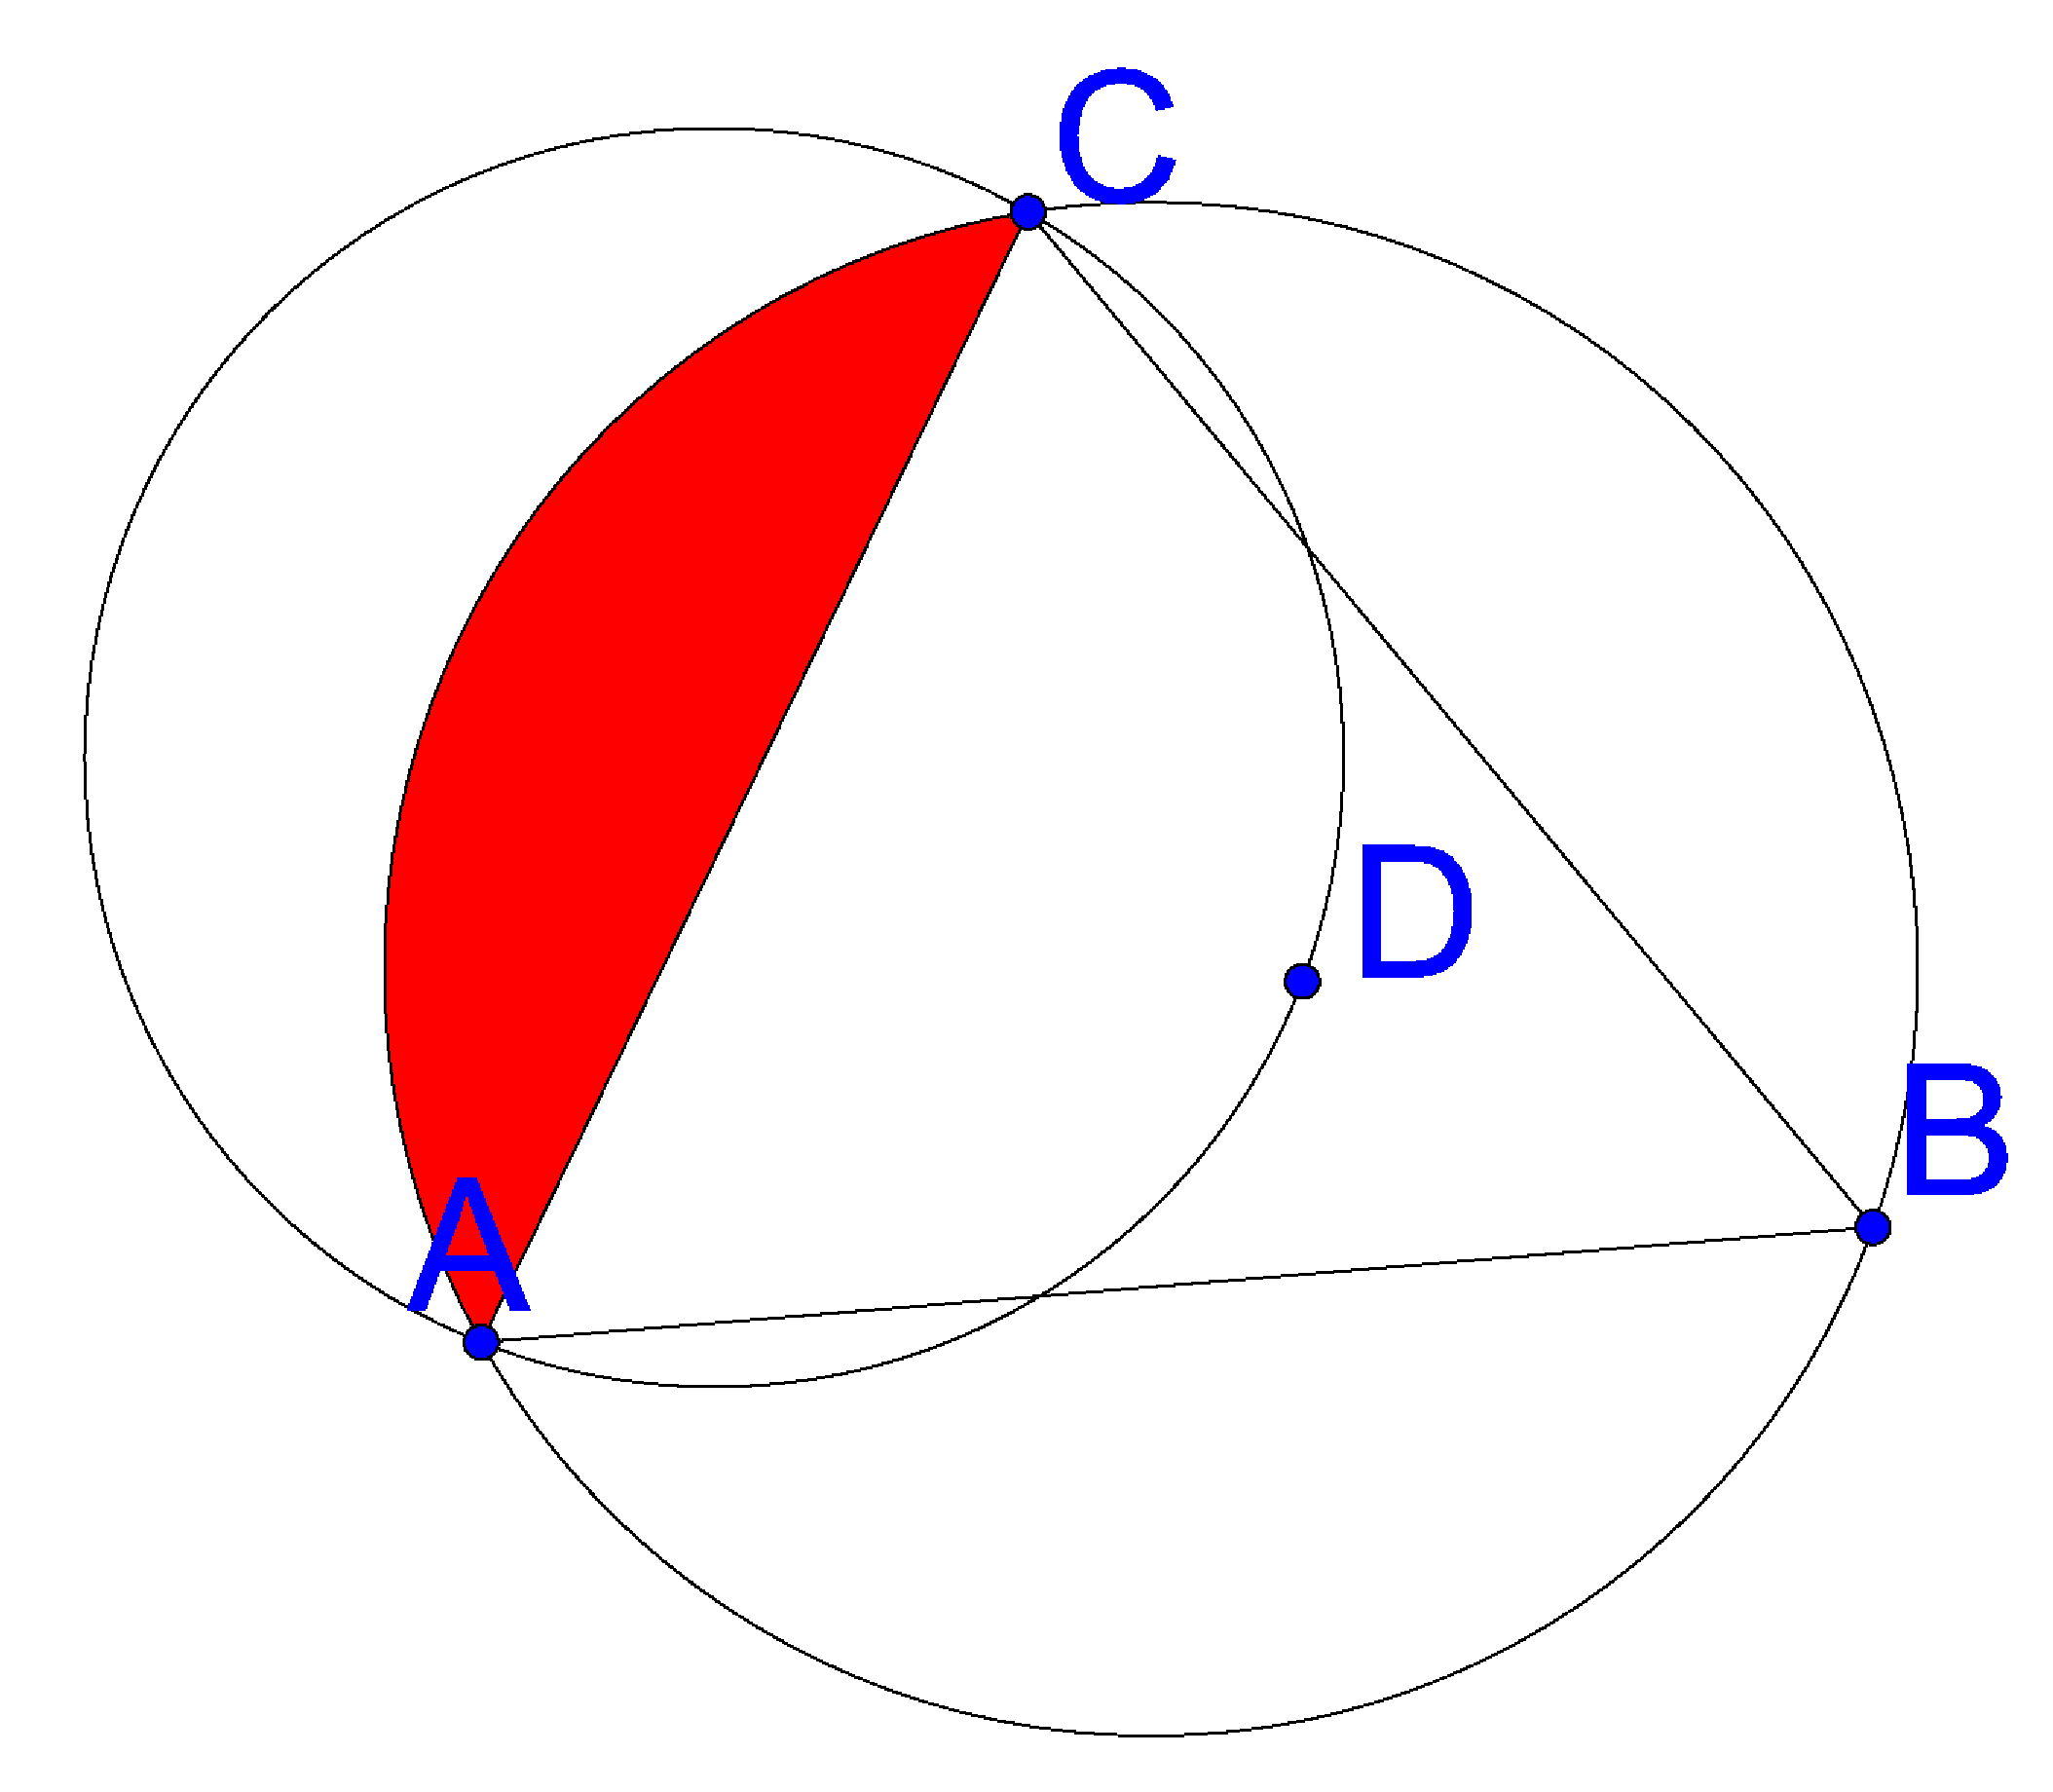
\includegraphics[width=0.2\linewidth]{eps/noPointinRegion.eps}
\caption{The red marked region contains no Points of G because it is always contained in $\bigcirc{ACD} $ which must be empty by definition.}
\label{fig:empty_region}
\end{figure}

Keil and Gutwin \cite{keil} proved the existence of a path between the points $A $ and $B $ and showed that the length of this path is delimited by the length of the arc from $A $ to $B $ on the circle $\bigcirc{ABC} $.
This path connects $A $ and $B $ when no other points of G are inside $\triangle{ABC} $.
The only precondition is that lemma \ref{emptyregion} holds (which it does).
This path is called the \emph{outward path}.
%überleitung

The recursive definition of this path taken from \cite{kanj} is as follows:
\begin{enumerate}
\item \textbf{Base case:} If $AB \in G $, the path consists of edge AB.
\item \textbf{Recursive step:} Otherwise, a point must reside in the region of $(O) $ subtended by chord AB and away from C. 
Let $T $ be such a point with the property that the region of $\bigcirc{ATB} $ subtended by chord $AB $ closer to $T $ is empty. 
We call T an \emph{intermediate point} with respect to the pair of points $(A, B) $.
Let $(O_1) $ be the circle passing through $A $ and $T $ whose center $O_1 $ lies on segment $AO $  and let $(O_2) $ be the circle passing through $B $ and $T $ whose center $O_2 $ lies on segment $BO $.
Then both $(O_1) $ and $(O_2) $ lie inside $(O) $, and $\angle{AO_1T} $ and $\angle{TO_2B} $ are both less than $\angle{AOB} \leq \frac{4\pi}{k} $.
Moreover, the region of $(O_1) $ subtended by chord $BT $ and containing $O_2 $ is empty. Therefore, we can recursively construct a path from $A $ to $T $ and a path from $T $ to $B $, and then concatenate them to obtain a path from A to B.  
\end{enumerate}
Figure \ref{fig:intermediate_point} contains an example for an intermediate point.


\begin{figure}[h!]
\centering
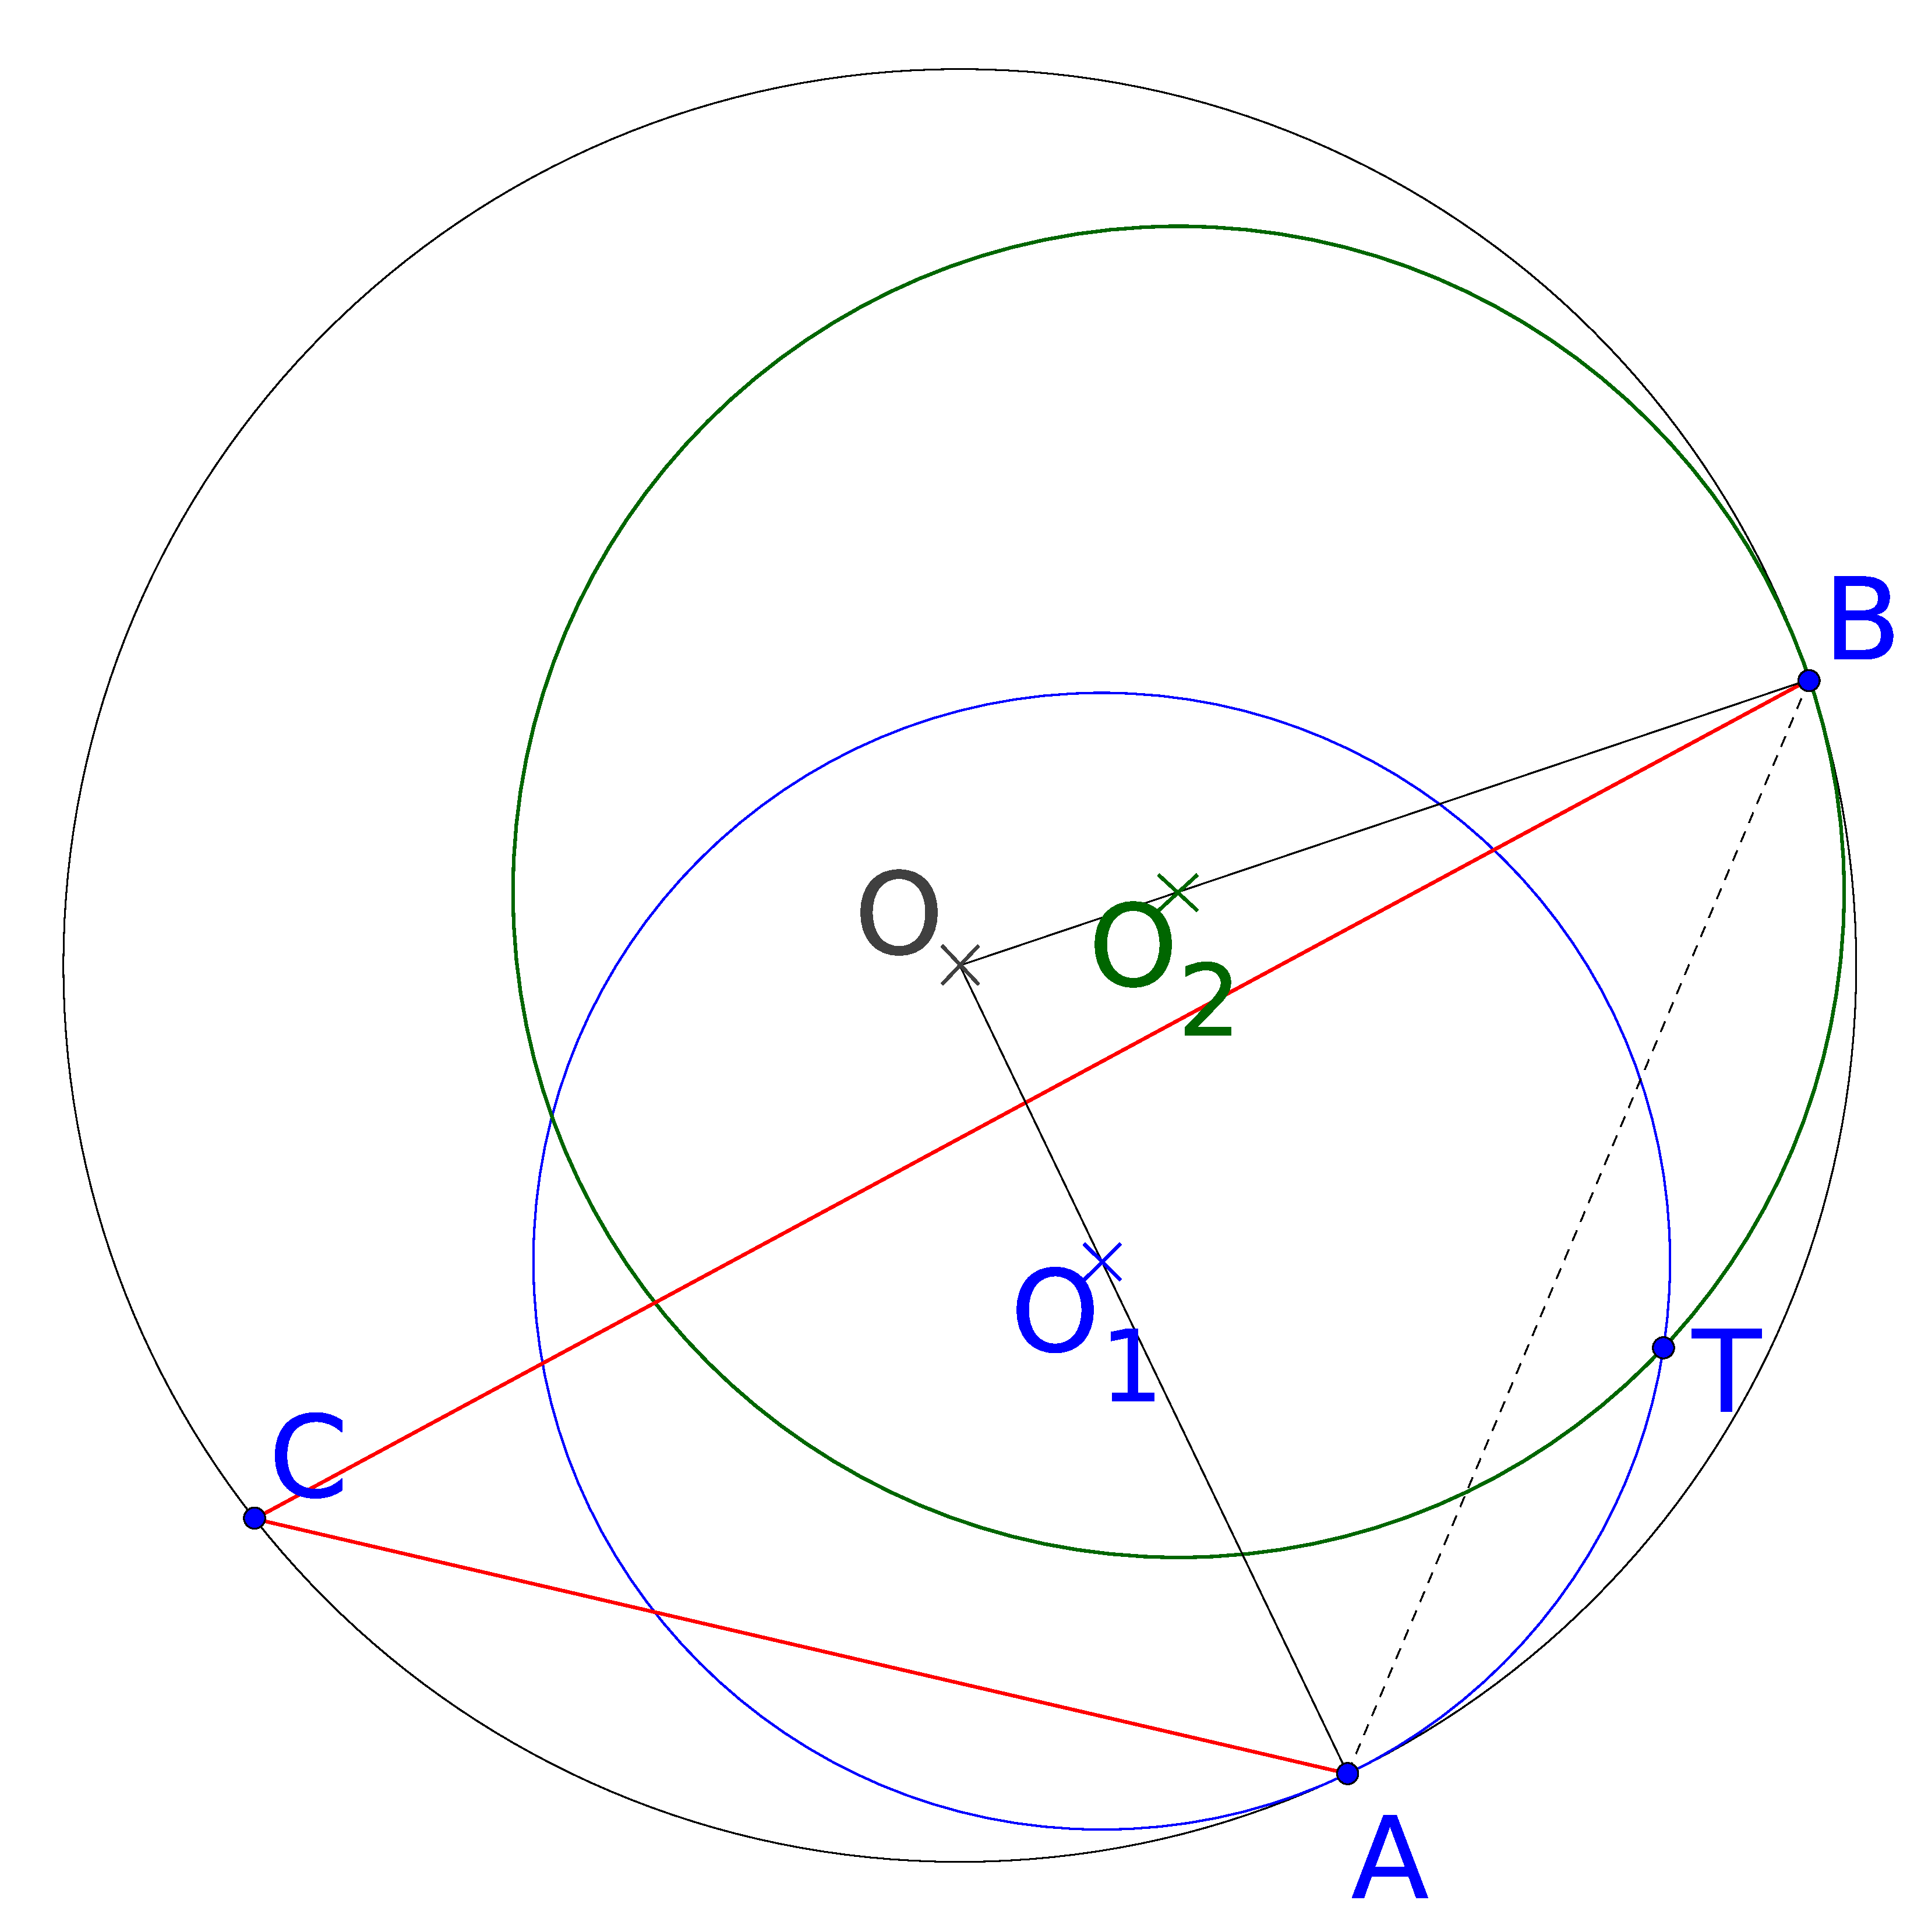
\includegraphics[width=0.5\linewidth]{eps/IntermediatePoint.eps}
\caption{The intermediate point $T $ with respect to pair $(A,B) $, and the circles $O_1 $ and $O_2 $, which are completely within $O $. }
\label{fig:intermediate_point}
\end{figure}


We must proof the following proposition (which is from \cite{kanj}).

\begin{prop}
\label{outward_path}
In every recursive step of the outward path construction described above, if $M_p $ is an intermediate point with respect to a pair of points $(M_i, M_j) $, then:
\begin{enumerate}
\item there is a circle passing through C and $M_p $ that contains no point of G, and
\item circles $\bigcirc{CM_iM_p} $ and $\bigcirc{CM_jM_p} $ contain no points of G, except, possibly, in the region subtended by chords $M_iM_p $ and $M_pM_j $, respectively, away from C.
\end{enumerate}
\end{prop}

\begin{figure}[h!]
\centering
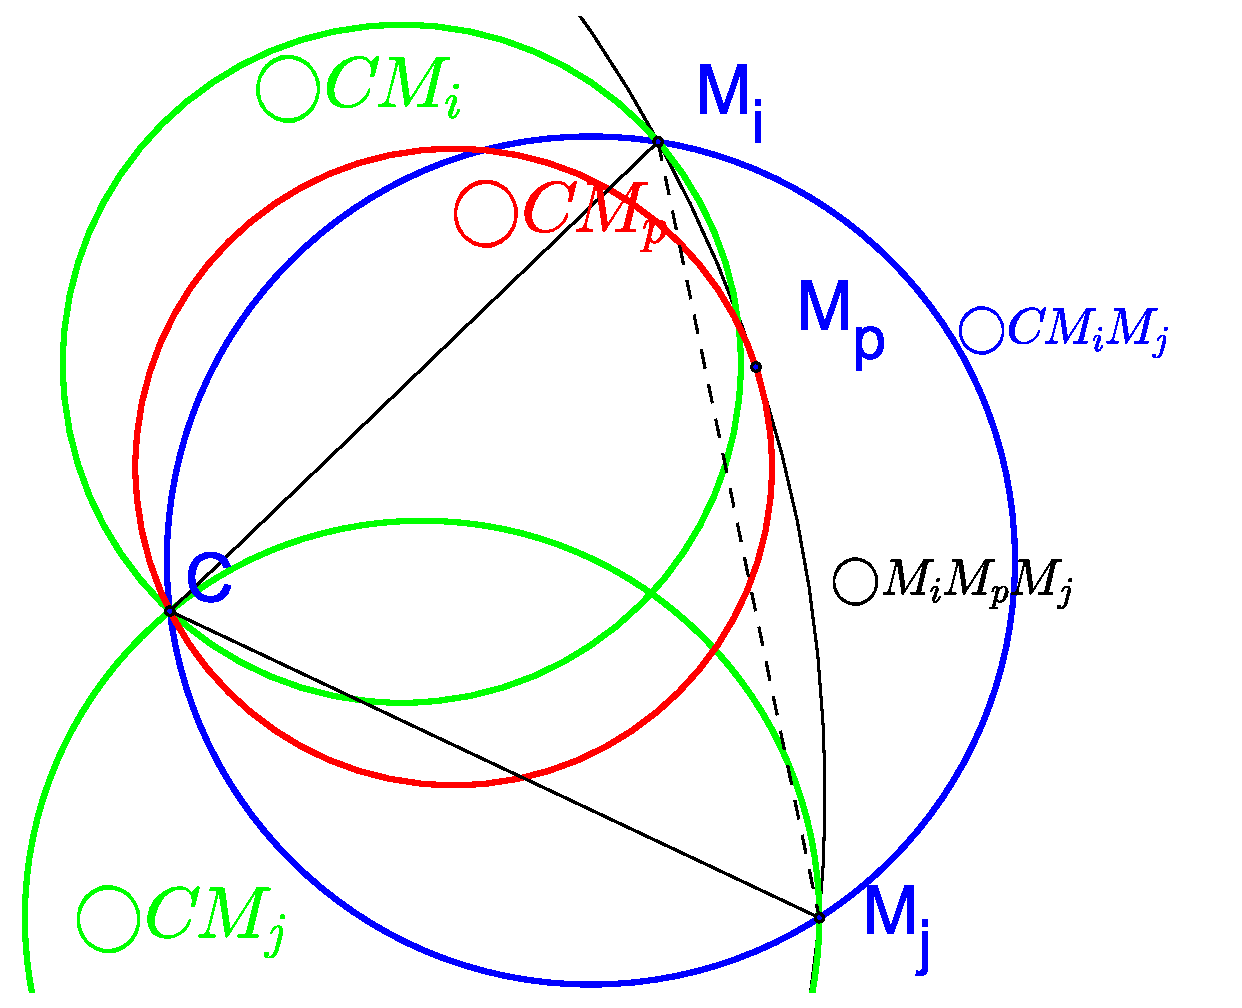
\includegraphics[width=0.9\linewidth]{eps/beweis_outward.eps}
\caption{Example for proof of proposition \ref{outward_path}.}
\label{fig:outward_path_beweis}
\end{figure}

\begin{proof}


Let $G $ be the set of nodes which is created by PDT. 
Since $CA $ and $CB $ are edges in $G $ there are circles $\bigcirc{CM_i} $ and $\bigcirc{CM_j} $ which have $C $ and $M_i $, and $C $ and $M_j $, respectively, on it's border and do not contain any other nodes of $G $. 
At this point I assume, without loss of generality, that $M_i $ and $M_j $ lie on the y-axis of the coordinate system and $C $ lies to the left of these points.
First, notice that $\triangle{CM_iM_j} $ is empty by precondition and the area $R_{\bigcirc{M_iM_pM_j}} $ of $\bigcirc{M_iM_pM_j} $ subtended by chord $M_iM_j $ away from $C $ contains no other points either.
This proof is divided into three cases.
\begin{enumerate}
\item $\bigcirc{CM_p} $ is tangential to $\bigcirc{CM_iM_j} $ at C.
\item $\bigcirc{CM_p} $ overlaps $\bigcirc{CM_iM_j} $ in the upper halfplane subtended by chord $CM_i $ (away from $M_j $).
\item $\bigcirc{CM_p} $ overlaps $\bigcirc{CM_iM_j} $ in the lower halfplane subtended by chord $CM_j $ (away from $M_i $).
\end{enumerate}
Since the two circles $\bigcirc{CM_p} $ and $\bigcirc{CM_iM_j} $ share the point $C $, $\bigcirc{CM_p} $ cannot overlap $\bigcirc{CM_iM_j} $ on both sides of the edge $CM_p $.
For case 1 $\bigcirc{CM_p} $ is completely inside $\bigcirc{CM_iM_j} $ and therefore devoid of any points.
For case 2 $\bigcirc{CM_p} $ is completely inside the area $R_{\bigcirc{M_iM_pM_j}} \cup \bigcirc{CM_iM_j} \bigcirc{CM_i} $ and, therefore, empty.
$\bigcirc{CM_p} $ cannot overlap $\bigcirc{CM_i} $ because of the following lemma.
\begin{lemma}
\label{circles}
If $A $ and $B $ are points in the plane and are located in different halfplanes of a line $CM_i $, and $A $ and $B $ are not allowed to reside inside a circle $\bigcirc{CM_i} $, there is no circle $\bigcirc{ABC} $ which does not contain $M_i $ and overlaps circle $\bigcirc{CM_i} $.
\end{lemma}
\begin{proof}
 Let, without loss of generality, $C $ and $M_i $ be on a line $CM_i $ which is parallel to the y-axis.
$A $ and $B $ are then located to the left and right of this line.
You can see this construction in figure \ref{fig:beweis_circles}.

This proof uses a contradiction. % widerspruchsbeweis  -> Florentin fragen
$A $ cannot reside inside $\bigcirc{CM_i} $, since $CM_i $ is a PDT-edge.
The circle $c_1 $ must not contain $M_i $ and, therefore, must cross the circle $\bigcirc{CM_i} $ in front of $M_i $.
Notice that the next part of the circle $c_1 $ must be inside of circle $\bigcirc{CM_i} $, since we started outside.
Because $c_1 $ must cross $B $ and $B $ lies outside of $\bigcirc{CM_i} $, $c_1 $ crosses a second time $\bigcirc{CM_i} $.
And the last conclusion is that $C $ is a common point of $\bigcirc{CM_i} $ and $c_1 $.
Hence, we have got three intersections of $\bigcirc{CM_i} $ and $c_1 $ at least.
Since $A $ and $B $ lie outside of $\bigcirc{CM_i} $, these two circles are not equal.
But two circles which intersect at least three times and are not equal, do not exist.
\end{proof}
The proof of case 3 works analogously.
These conclusions proof part a) of proposition \ref{outward_path}.

The following part of this work proofs part b) of the same proposition.
The main argument of this proof is that $\bigcirc{CM_iM_p} $ is contained completely in the area $\bigcirc{CM_i} \cup  R_{\bigcirc{M_iM_pM_j}} \cup R2_{\bigcirc{CM_iM_j}} $ with $R2_{\bigcirc{CM_iM_j}} $ being the area of $\bigcirc{CM_iM_j} $ subtended by chord $M_iM_j $ closer to $C $.
I show that every possible position of $\bigcirc{CM_i} $ includes the area $R3_{\bigcirc{CM_iM_p}} $ of $\bigcirc{CM_iM_p} $ subtended by chord $CM_i $ away from $M_j $.
The proof is divided into three cases of how $\bigcirc{CM_i} $ can be located:
\begin{enumerate}
\item $\bigcirc{CM_i} $ is equal to $\bigcirc{CM_iM_p} $.
\item $\bigcirc{CM_i} $ overlaps $\bigcirc{CM_iM_p} $ in the halfplane subtended from line $CM_i $ away from $M_j $.
\item $\bigcirc{CM_i} $ overlaps $\bigcirc{CM_iM_p} $ in the halfplane subtended from line $CM_i $ closer to $M_j $.
\end{enumerate}
First, assume, without loss of generality, that $C $ and $M_i $ lie on a horizontal line and $M_j $ is located below this line.
$\bigcirc{CM_iM_p} $ can only overlap $\bigcirc{CM_i} $ on one side of line $CM_i $, since they share these two points.

For case 1, since $\bigcirc{CM_i} $ is empty, $\bigcirc{CM_iM_p} $ must be empty, too.

For case 2, $\bigcirc{CM_i} $ moves up, away from $M_j $, expanding the area in the same direction of which $R3_{\bigcirc{CM_iM_p}} $ is located.
So, $R3_{\bigcirc{CM_iM_p}} $ cannot overlap $\bigcirc{CM_i} $ in this case.

Case 3, the only case where $R3_{\bigcirc{CM_iM_p}} $ would overlap $\bigcirc{CM_i} $, cannot occur, since $M_p \in G $ and $M_p $ is, obviously, located on $\bigcirc{CM_iM_p} $.
So, if $\bigcirc{CM_i} $ moves down, towards $M_j $, it would contain $M_p $, which cannot happen, since $\bigcirc{CM_i} $ is a PDT-circle. 

Notice that the proof for $\bigcirc{CM_jM_p} $ works analogously substituting $M_i $ with $M_j $ and vice versa.
 
\end{proof}
\begin{figure}[h!]
\centering
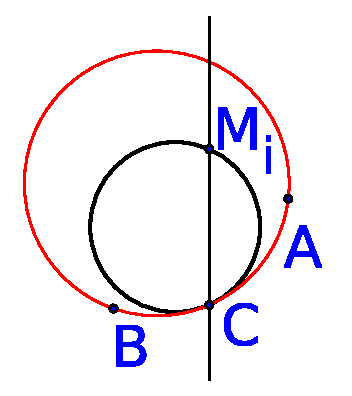
\includegraphics[width=0.5\linewidth]{eps/beweis_circles.eps}
\caption{Example of the construction of lemma \ref{circles}.}
\label{fig:beweis_circles}
\end{figure}
Another lemma we need in order to proof proposition \ref{mastertheorem} is the following:
\begin{lemma}
\label{outward_3}
If four points $A $, $B $, $C $ and $M_1 $ are on one circle and $C $ and $M_1 $ are on different halfplanes of chord $AB $, then $\angle{AM_1B} + \angle{ACB} =\pi $ is true (see figure \ref{fig:winkel_fuer_outward_3} for an graphical illustration of this lemma).
\end{lemma}
\begin{proof}
see Euklid, book 3, Proposition 22.  (Nochmal besprechen)


\begin{figure}[h!]
\centering
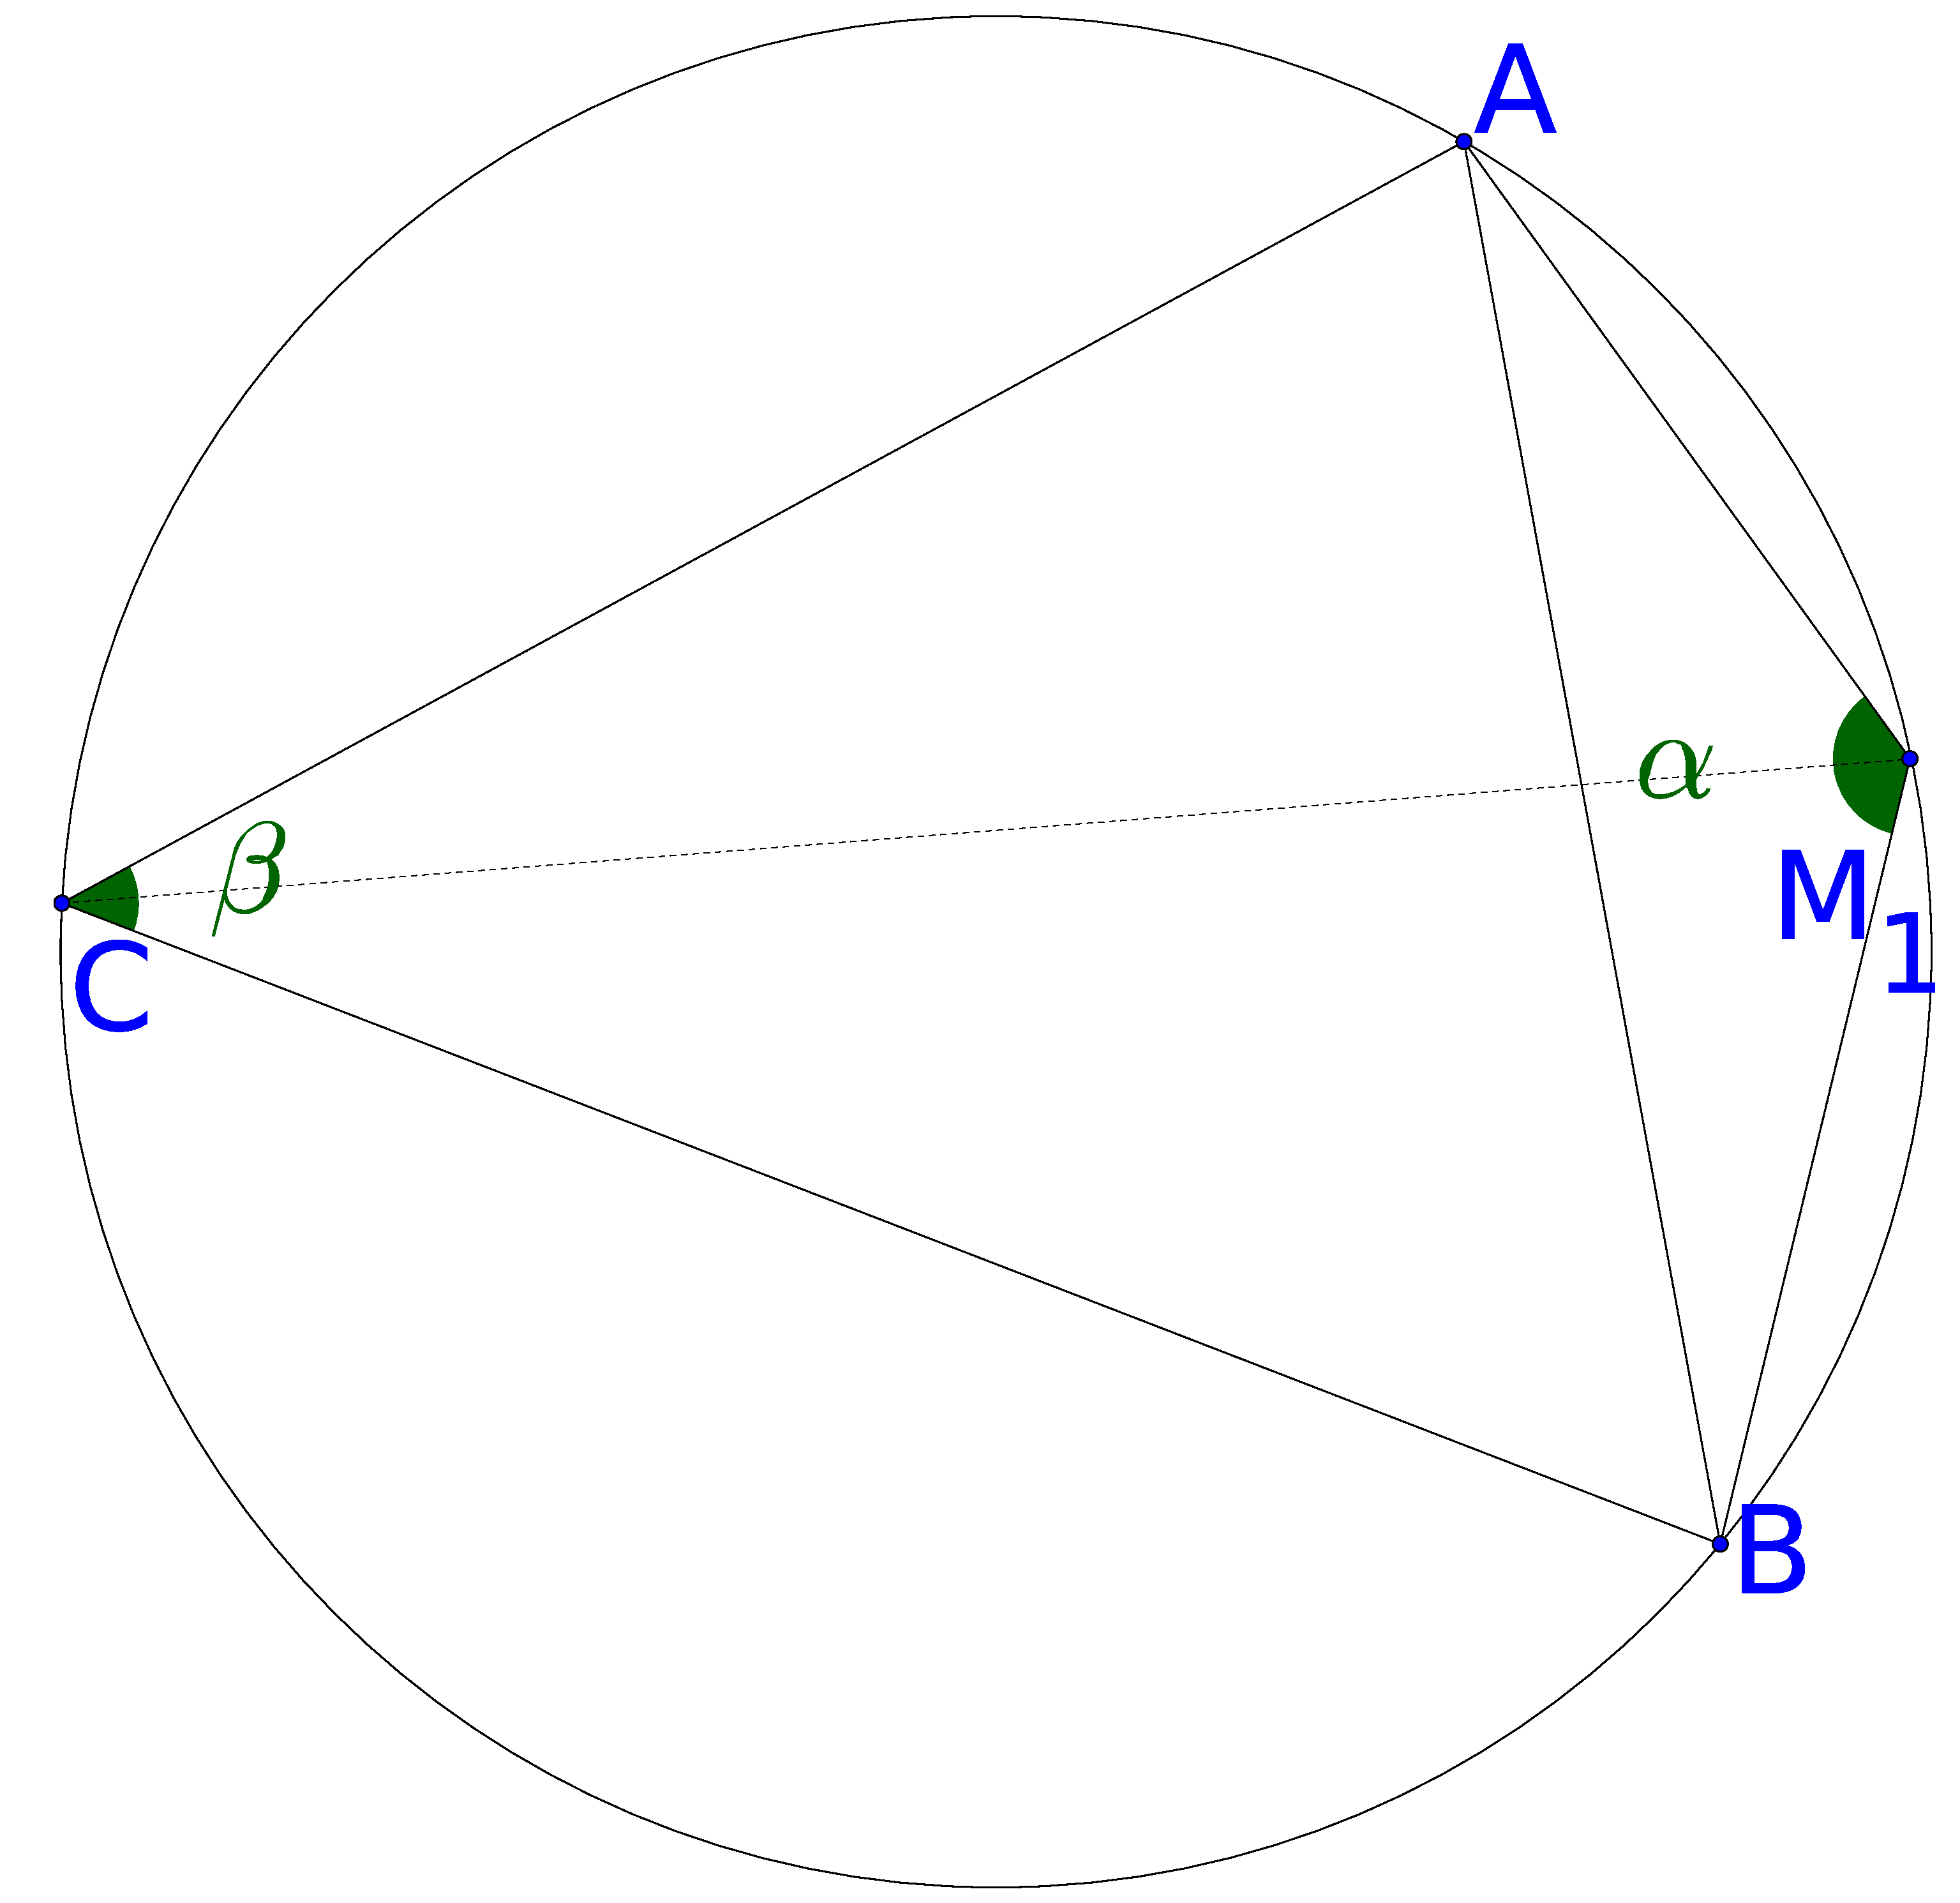
\includegraphics[width=0.4\linewidth]{eps/Winkel_fuer_outward_3.eps}
\caption{Example for lemma \ref{outward_3} }
\label{fig:winkel_fuer_outward_3}
\end{figure}
\end{proof}
Now, we can proof the following lemma from \cite{kanj}, which shows, that for the case of the outward path, proposition \ref{mastertheorem} is satisfied:

\begin{lemma}
Let $k \geq 14$ be an integer, and let $CA $ and $CB $ be edges in $G $ such that $\angle{BCA} \leq \frac{2\pi}{k} $ and $CA $ is the shortest edge in the angular sector $\angle{BCA} $. There exists a path $p : A=M_0, M_1, \dotsc, M_r=B $ in $G $ such that:
\begin{enumerate}
\renewcommand{\labelenumi}{(\roman{enumi})}
\item $|CA| + \sum_{i=0}^{r-1}|M_iM_{i+1}| \leq (1+2\pi(k \cos(\frac{\pi}{k}))^{-1})|CB|$
\item There is no edge in $G $ between any pair $M_i $ and $M_j $ lying in the closed region delimited by $CA, CB $ and the edges of $p $, for any $i $ and $j $ satisfying $0 \leq i < j -1 \leq r $.
\item $\angle{M_{i-1}M_iM_{i+1}} > \pi - \frac{2\pi}{k} $, for $i=1,\dotsc,r-1 $.
\item $\angle{CAM_1} \geq \frac{\pi}{2} - \frac{pi}{k} $.
\end{enumerate}	 
\end{lemma}

\begin{proof}
This proof is performed almost equal to \cite{kanj}, but covering more details.
%and $\sin{\theta} = \frac{|AB|}{2|OA|}) $
\renewcommand{\labelenumi}{(\roman{enumi})}%
\begin{enumerate}
\item 
\begin{equation*}
\begin{split}
|CA|+|\overarc{AB}| &= |CB| + 2\theta \cdot |OA| \\
&\stackrel{a)}{=}|CB| + (\frac{\theta}{\sin{\theta}})\cdot |AB| \\
&\stackrel{b)}{=} |CB| + (\frac{\theta}{\cos{\frac{\theta}{2}}}) \cdot |CB|\\
&\stackrel{c)}{\leq} (1+2\pi(k \cos{\frac{\pi}{k}})^{-1}) |CB|  
\end{split}
\end{equation*}
Since $|CA| \leq |CB| $, $|CA|+|\overarc{AB}| $ is largest, when $CA $ and $CB $ are symmetrical to the diameter of $\bigcirc{ABC} $, we can assume $|CA|=|CB| $.
$|\overarc{AB}| $ can be replaced with $2\theta \cdot |OA| $ (angle times radius).
For every chord $s $ of a circle $(c) $ it is true, that $s=2r\sin{\frac{\alpha}{2}} $, with $r $ being the radius of $(c) $ and $\alpha $ being the angle between the endpoints of $s $ in middlepoint $c $ facing $s $.
Note that $\alpha = 2\theta $. 
These equations proof a).

Next, substitute $|AB| $ with $|AB| = \sin{\frac{\theta}{2}} \cdot 2|CB| $ and replace $\sin{\theta} $ with the trigonometry identity $\sin{\theta}=2\sin{\frac{\theta}{2}} \cos{\frac{\theta}{2}} $.
You receive equation b).

At last, substitute $\theta $ using inequality $\theta \leq \frac{2\pi}{k} $ with $k > 2 $, obtaining c).

\item  Suppose, $M_i $ and $M_j $ is an edge in $G $, then there exists a circle with these two points on it's border which does not contain any other node of $G $.
So, $M_p $ must lie outside of this circle.
By proposition \ref{outward_path} part a) there is a circle $\bigcirc{CM_p} $ trough $C $ and $M_p $ which is empty.
These two last observations contradict each other, since $\bigcirc{M_iM_j} $ would always contain $M_p $.
If $M_p $ does not reside in the circle $\bigcirc{M_iM_j} $, this circle and the circle $\bigcirc{CM_p} $ would cross at least three times (and are not equal), which cannot exist.

\item Since the angles $\alpha $ and $\beta $ between opposite points of a chord in a rectangle which corners lie on a circle are supplementary, this is a fact: $\angle{AM_1B}=\pi - \angle{ACB} $ (see lemma \ref{outward_3} for more details).
The angle $\angle{M_{i-1}CM_{i+1}} $ is smallest, if $M_{i-1} $ and $M_{i+1} $ lie on the circle. 
Note, by precondition we assume $\angle{BCA} \leq \frac{2\pi}{k} $.
These facts proof following inequalities:
\begin{equation*}
\begin{split}
 \angle{M_{i-1}M_iM_{i+1}}&\geq \pi - \angle{M_{i-1}CM_{i+1}}\\
 &\geq \pi - \angle{BCA} \\ &\geq \pi - \frac{2\pi}{k}\\
\end{split}
\end{equation*}



 %http://www.regentsprep.org/regents/math/geometry/gp15/circleangles.htm
\item Since $M_1 $ is inside the area subtended by chord $AB $ from $\bigcirc{ABC} $ \emph{away} from $C $, it is true that $\angle{CAM_1} \geq \angle{CAB} \geq \frac{\pi}{2} -\frac{\pi}{k} $.
The last inequality is true because:
 \begin{equation*}
  \begin{split}
   \angle{CAB}+\angle{ABC}+\underbrace{\angle{BCA}}_{\leq \frac{2\pi}{k}}&=\pi\\
   \angle{CAB}+\angle{ABC} &\geq \pi - \frac{2\pi}{k} \\
   \angle{CAB} &\geq \frac{\pi-\frac{2\pi}{k}}{2}=\frac{\pi}{2}-\frac{\pi}{k}
   \end{split} 
\end{equation*}
Since $CA \leq CB $, $\angle{CAB} $ can be at most the half of $\pi - \frac{2\pi}{k} $, proving the last inequality.

\end{enumerate}
\end{proof}

 
%\begin{figure}[h!]
%\centering
%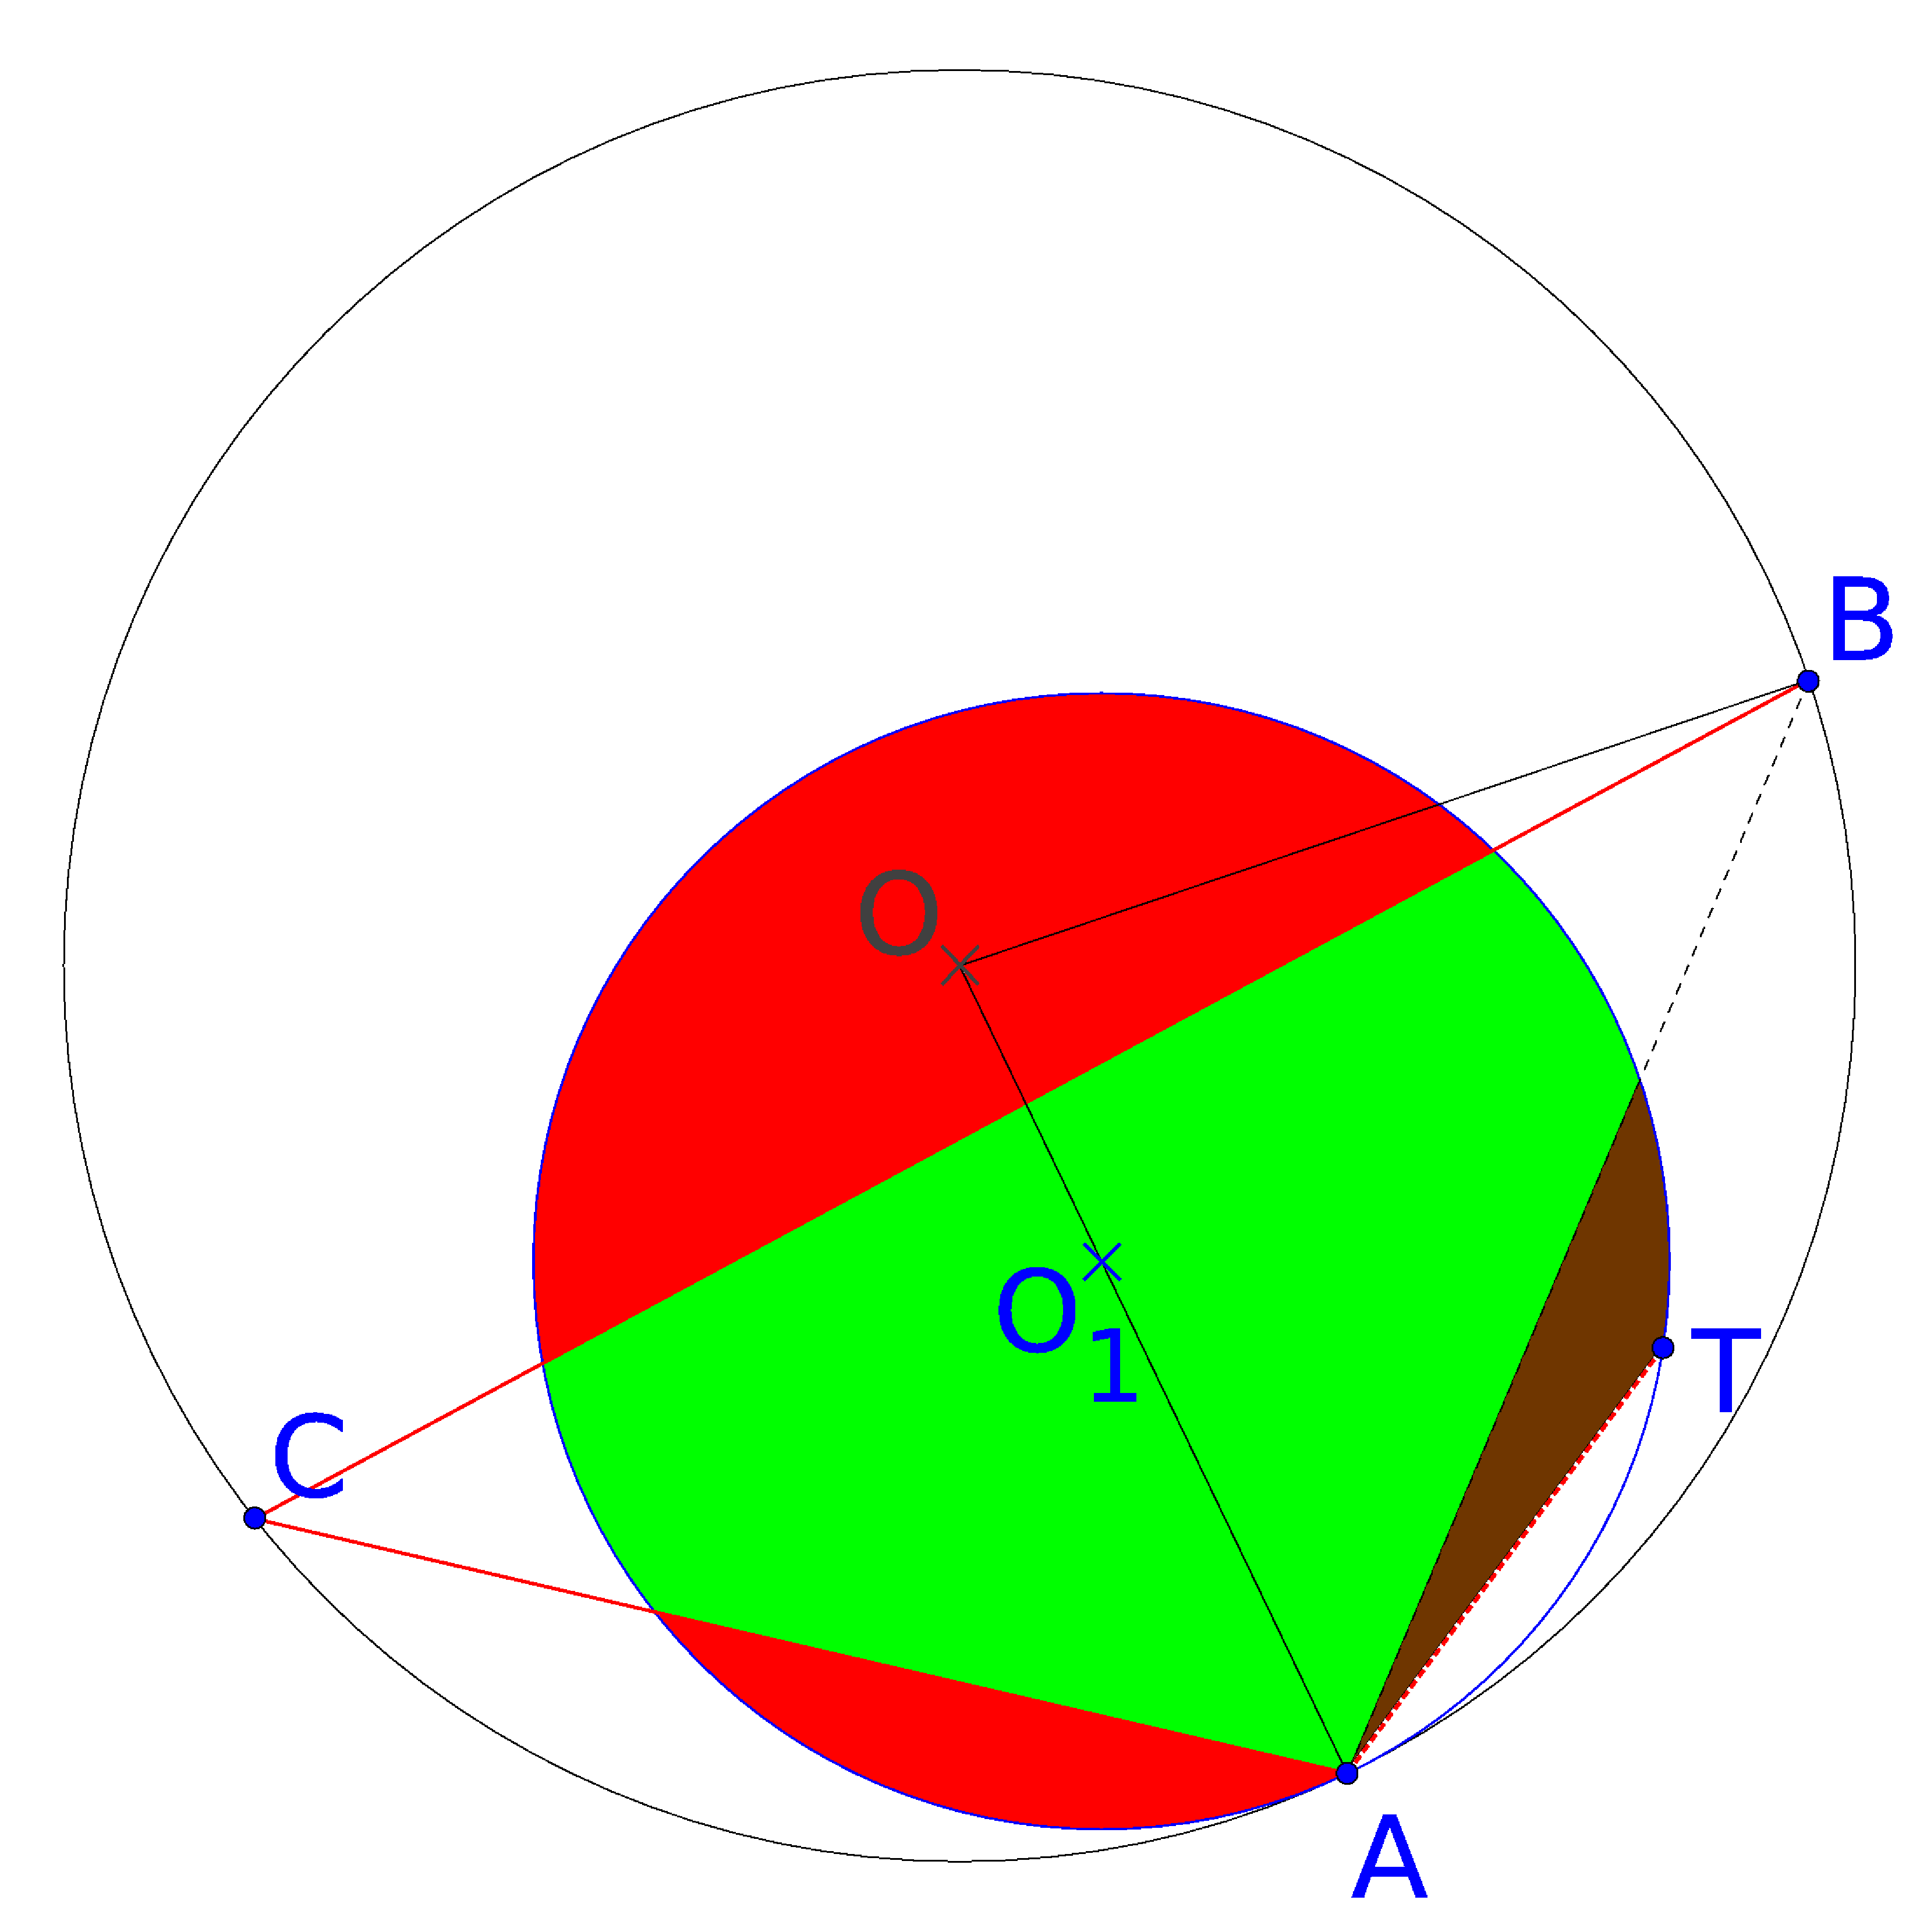
\includegraphics[width=0.5\linewidth]{eps/IntermediatePoint_beweis.eps}
%\caption{The red regions must be empty by lemma \ref{emptyregion}, the green area is empty by precondition and the brown region must be empty by ... }
%\label{fig:intermediate_point_beweis}
%\end{figure}
%
%
%\begin{enumerate}
%\item $|CA| + \sum\nolimits_{i=0}^{r-1} |M_iM_{i+1}| \leq (1+2\pi (k*\cos{\frac{\pi}{k}})^{-1})|CB| $
%\item There is no edge in G between any pair $M_i $ and $M_j $ lying in the closed region delimited by CA, CB and the edges of p, for any i and j satisfying $0 \leq i < j-1 \leq r $ 
%\item $\angle{M_{i-1}M_iM_{i+1}} > \frac{k-2}{k}\pi $, for $i=1, ..., r-1 $ 
%\item $\angle{CAM_1} \geq \frac{\pi}{2}-\frac{\pi}{k} $
%\end{enumerate}




\subsection{inward Path}
Now, we perform the proof for the case when $\triangle{ABC} $ contains other nodes.

Let $S $ be the set of points which contains points $A $ and $B $, and all the points interior to $\triangle{ABC} $ excluding $C $.
Then $CH(S) $ are all the points which are on the convex hull of $S $.
Let these points be called $N_0=A $ and $N_t=B $ and points $N_1 , \cdots ,N_{t-1} $ are the points on $CH(S) $ which lie inside $\triangle{ABC} $. 
The following proposition is taken from \cite{kanj}:
\begin{prop}
\label{inward_pre}
For every $i=1, \cdots, t-1: $
\begin{enumerate}
\renewcommand{\labelenumi}{\alph{enumi})}
\item $CN_i \in G $,
\item $|CN_i| \leq |CN_{i+1}| $, and
\item  $\angle{N_{i-1}N_iN_{i+1}} \geq \pi $, where $\angle{N_{i-1}N_iN_{i+1}} $ is the angle facing point $C $.
\end{enumerate} 
\end{prop}
\begin{proof}
Since $CA $ is the shortest edge in the angular sector $\angle{BCA} $, $|CA| \leq CN_i , for i=1 ,\cdots, t-1 $  and since $N_1 , \cdots, N_t $ are on $CH(S) $, b) is true.

Part c) follows from the convexity of $CH(S) $. All interior angles to $CH(S) $ measure at most $\pi $, so all the exterior angles fulfil $\angle{N_{i-1}N_iN_{i+1}}\geq \pi $ 
\end{proof}

Since $CN_i \leq CN_{i+1} $ and no other point of $G $ lies inside $\triangle{N_iCN_{i+1}} $, $CN_i $ is the shortest edge in the angular sector $\angle{N_iCN_{i+1}} $.
\include{reactive_Construction}
%related work: kanj hat neues ergebnis mit knotenbeschränkung kleiner gleich 11...
%improved local algorithms   2012
\section{Conclusion}
RMYS is due to its reactivity a robust algorithm to construct a bounded degree, planar graph which is most likely an Euclidean spanner.
As for now, it is not appropriate to use it to create a local view on just one node in consequence of the message overhead it creates.
However, it is well suited to create a complete graph in a reactive way while providing a constant node degree on top of planarity and a constant spanning ratio.
RMYS is the first algorithm which inherits all these graph properties and is created in a reactive way.

For the past years reactivity in ad hoc sensor networks reduced permanently the message overhead to create planar graphs which later turned out to be spanners.
In addition, it is now possible to append the property of a constant node degree for each node in the graph to reactive approaches.
This saves additional messages if a routing protocol uses the underlying RMYS graph.

In order to minimize the constant node degree bound of $14 $ further research should focus on formally proving the spanning ratio of RMYS and check whether it is possible to lower the degree bound without increasing the spanning ratio significantly.
Another interesting point for future research is to reduce the message overhead for RMYS when it is executed on one node.
For instance, under the condition that all possibilities where RMYS creates a uni directional edge are known (refer to figures \ref{fig:RMYS_case_one_cone_empty} and \ref{fig:RMYS_case_error_bidirectional} for help in this matter) one can possibly omit the last broadcast completely.
Instead, one must find a pattern for each of these possibilities to detect uni directional edges without sending additional messages.
\include{Programming}

\begin{appendix}
%% include your appendices here
%\include{appendix-A}
\end{appendix}
%%%%%%%%%%%%%%%%%%%%%%%%%%%%%%%%%%%%%%%%%%%%%%%%%%%%%%%%%%%%%%%%%
%%%%%%%%%%%%%%%%%%%%%%%%%%%%%%%%%%%%%%%%%%%%%%%%%%%%%%%%%%%%%%%%%
%\addcontentsline{toc}{chapter}{Bibliography}
\bibliographystyle{unsrt}
{\footnotesize\bibliography{BachelorarbeitTim}}
\end{document}
%%%%%%%%%%%%%%%%%%%%%%%%%%%%%%%%%%%%%%%%%%%%%%%%%%%%%%%%%%%%%%%%%
%%%%%%%%%%%%%%%%%%%%%%%%%%%%%%%%%%%%%%%%%%%%%%%%%%%%%%%%%%%%%%%%%
\endinput
%%
%% End
